\mfpicnumber{1}

\opengraphsfile{CircularFunctions}

\setcounter{footnote}{0}

\label{CircularFunctions}

In section \ref{TheUnitCircle},  we defined $\cos(\theta)$ and $\sin(\theta)$  for angles $\theta$ using the coordinate values of points on the Unit Circle.  As such, these functions earn the moniker \index{circular function}\index{function ! circular}\textbf{circular functions}.\footnote{In Theorem \ref{cosinesinetriangle} we also showed cosine and sine to be functions of an angle residing in a right triangle so we could just as easily call them \emph{trigonometric} functions.  In later sections, you will find that we do indeed use the phrase `trigonometric function' interchangeably with the term `circular function'.} It turns out that cosine and sine are just two of the six commonly used circular functions which we define below. 

\enlargethispage{.2in}

%\medskip

\colorbox{ResultColor}{\bbm

\begin{defn} \label{circularfunctions}  \textbf{The Circular Functions:} Suppose $\theta$ is an angle plotted in standard position and $P(x,y)$ is the point on the terminal side of $\theta$ which lies on the Unit Circle.  

\begin{itemize}

\item The \index{cosine ! of an angle} \textbf{cosine} of $\theta$, denoted $\cos(\theta)$, is defined by $\cos(\theta) = x$.

\item The \index{sine ! of an angle} \textbf{sine} of $\theta$, denoted $\sin(\theta)$, is defined by $\sin(\theta) = y$.

\item The \index{secant ! of an angle} \textbf{secant} of $\theta$, denoted $\sec(\theta)$, is defined by $\sec(\theta) = \dfrac{1}{x}$, provided $x \neq 0$.

\item The \index{cosecant ! of an angle} \textbf{cosecant} of $\theta$, denoted $\csc(\theta)$, is defined by $\csc(\theta) = \dfrac{1}{y}$, provided $y \neq 0$.

\item The \index{tangent ! of an angle} \textbf{tangent} of $\theta$, denoted $\tan(\theta)$, is defined by $\tan(\theta) = \dfrac{y}{x}$, provided $x \neq 0$.

\item The \index{cotangent ! of an angle} \textbf{cotangent} of $\theta$, denoted $\cot(\theta)$, is defined by $\cot(\theta) = \dfrac{x}{y}$, provided $y \neq 0$.

\end{itemize}

\end{defn}

\ebm}

\vspace{0.1in}

While we left the history of the name `sine' as an interesting research project in Section \ref{TheUnitCircle}, the names `tangent' and `secant' can be explained using the diagram below.  Consider the acute angle $\theta$ below in standard position. Let $P(x,y)$ denote, as usual,  the point on the terminal side of $\theta$ which lies on the Unit Circle and let $Q(1,y')$ denote the point on the terminal side of $\theta$ which lies on the vertical line $x=1$. 

\vspace{-0.1in}
\begin{center}

\begin{mfpic}[25]{-1}{7}{-1}{7}
\axes
\drawcolor[gray]{0.7}
\parafcn{0,90,5}{3*dir(t)}
\drawcolor[rgb]{0.33,0.33,0.33}
\arrow \parafcn{5, 55, 5}{0.75*dir(t)}
\tlabel[cc](0.75,0.5){\scriptsize $\theta$}
\point[3pt]{(0,0), (1.5, 2.5981), (3,5.196), (3,0), (1.5,0)}
\tlabel(6.75,-0.5){\scriptsize $x$}
\tlabel(0.25,6.75){\scriptsize $y$}
\tlabel(0.25,3.1){\scriptsize $1$}
\tlabel(-0.5,-0.5){\scriptsize $O$}
\tlabel(2.75,-0.5){\scriptsize $B(1,0)$}
\tlabel(1.25, -0.5){\scriptsize $A(x, 0)$}
\xmarks{0 step 3 until 3}
\ymarks{0 step 3 until 3}
\arrow \polyline{(0,0), (4,6.9282)}
\polyline{(3,0), (3,5.196)}
\polyline{(2.75,0), (2.75, 0.25), (3,0.25)}
\polyline{(1.5,0), (1.5, 2.5981)}
\polyline{(1.25,0), (1.25,0.25), (1.5,0.25)}
\tlabel(1.75,2.6){\scriptsize $P(x,y)$}
\tlabel(3.25,5.25){\scriptsize $Q(1,y') = (1, \tan(\theta))$}
\end{mfpic} 

\end{center}

%\medskip

The word `tangent' comes from the Latin meaning `to touch,' and for this reason, the line $x=1$ is called a \textit{tangent} line to the Unit Circle since it intersects, or `touches', the circle at only one point, namely $(1,0)$.  Dropping perpendiculars from $P$ and $Q$ creates a pair of similar triangles $\Delta OPA$ and $\Delta OQB$.  Thus $\frac{y'}{y} = \frac{1}{x}$ which gives  $y' = \frac{y}{x} = \tan(\theta)$, where this last equality comes from applying Definition  \ref{circularfunctions}. We have just shown that for acute angles $\theta$, $\tan(\theta)$ is the $y$-coordinate of the point on the terminal side of $\theta$ which lies on the line $x = 1$ which is \textit{tangent} to the Unit Circle. Now the word `secant' means `to cut', so a secant line is any line that `cuts through' a circle at two points.\footnote{Compare this with the definition given in Section \ref{LinearFunctions}.}  The line containing the terminal side of $\theta$ is a secant line since it intersects the Unit Circle in Quadrants I and III.   With the point $P$ lying on the Unit Circle, the length of the hypotenuse of $\Delta OPA$ is $1$. If we let $h$ denote the length of the hypotenuse of $\Delta OQB$, we have from similar triangles that $\frac{h}{1} = \frac{1}{x}$, or $h = \frac{1}{x} = \sec(\theta)$.  Hence for an acute angle $\theta$, $\sec(\theta)$ is the length of the line segment which lies on the secant line determined by the terminal side of $\theta$ and `cuts off' the tangent line $x=1$.  Not only do these observations help explain the names of these functions, they serve as the basis for a fundamental inequality needed for Calculus which we'll explore in the Exercises.

\smallskip 

Of the six circular functions, only cosine and sine are defined for all angles.  Since $\cos(\theta) = x$ and $\sin(\theta) = y$ in Definition \ref{circularfunctions}, it is customary to rephrase the remaining four circular functions in terms of cosine and sine.  The following theorem is a result of simply replacing $x$ with $\cos(\theta)$ and $y$ with $\sin(\theta)$ in Definition \ref{circularfunctions}.

\smallskip

\colorbox{ResultColor}{\bbm

\begin{thm} \label{recipquotid}  \textbf{Reciprocal and Quotient Identities:} \index{Reciprocal Identities} \index{Quotient Identities} 

\begin{itemize}

\item $\sec(\theta) = \dfrac{1}{\cos(\theta)}$, provided $\cos(\theta) \neq 0$;  if $\cos(\theta) = 0$, $\sec(\theta)$ is undefined.

\item $\csc(\theta) = \dfrac{1}{\sin(\theta)}$, provided $\sin(\theta) \neq 0$;  if $\sin(\theta) = 0$, $\csc(\theta)$ is undefined.

\item $\tan(\theta) = \dfrac{\sin(\theta)}{\cos(\theta)}$, provided $\cos(\theta) \neq 0$;  if $\cos(\theta) = 0$, $\tan(\theta)$ is undefined.

\item $\cot(\theta) = \dfrac{\cos(\theta)}{\sin(\theta)}$, provided $\sin(\theta) \neq 0$;  if $\sin(\theta) = 0$, $\cot(\theta)$ is undefined.

\end{itemize}

\end{thm}

\ebm}

\medskip

It is high time for an example.

\begin{ex} \label{circularfunctionsex}  Find the indicated value, if it exists.

\begin{multicols}{3}

\begin{enumerate}

\item  $\sec\left(60^{\circ}\right)$

\item  $\csc\left(\frac{7 \pi}{4} \right)$

\item  $\cot(3)$

\setcounter{HW}{\value{enumi}}

\end{enumerate}

\end{multicols}

\begin{enumerate}

\setcounter{enumi}{\value{HW}}

\item $\tan\left(\theta\right)$, where $\theta$ is any angle coterminal with $\frac{3\pi}{2}$.

\item $\cos\left(\theta\right)$, where $\csc(\theta) = -\sqrt{5}$ and $\theta$ is a Quadrant IV angle.

\item $\sin\left(\theta\right)$, where $\tan(\theta) = 3$ and $\pi < \theta < \frac{3\pi}{2}$.

\end{enumerate}

{\bf Solution.}  

\begin{enumerate}

\item  According to Theorem \ref{recipquotid},   $\sec\left(60^{\circ}\right) = \frac{1}{\cos\left(60^{\circ}\right)}$. Hence,  $\sec\left(60^{\circ}\right) = \frac{1}{(1/2)} = 2$.

\item  Since $\sin\left( \frac{7\pi}{4}\right) = - \frac{\sqrt{2}}{2}$,  $\csc\left( \frac{7\pi}{4}\right) = \frac{1}{\sin\left( \frac{7\pi}{4}\right)} = \frac{1}{- \sqrt{2}/2} = - \frac{2}{\sqrt{2}} = - \sqrt{2}$.

\item  Since $\theta = 3$ radians is not one of the `common angles' from Section \ref{TheUnitCircle}, we resort to the calculator for a decimal approximation.  Ensuring that the calculator is in radian mode, we find $\cot(3) = \frac{\cos(3)}{\sin(3)} \approx -7.015$.

\begin{tabular}{cc}

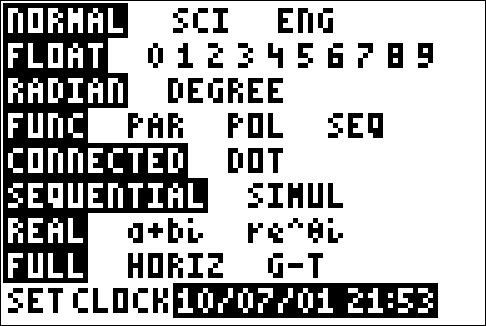
\includegraphics[width=2in]{./IntroTrigGraphics/CircularFunctions01.jpg} &
\hspace{0.75in} 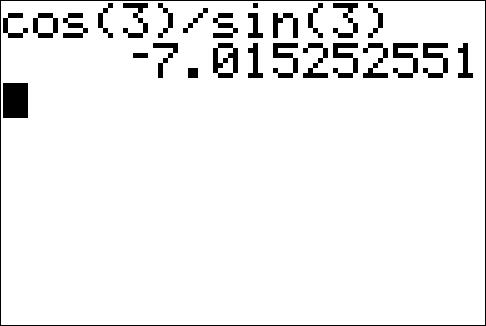
\includegraphics[width=2in]{./IntroTrigGraphics/CircularFunctions02.jpg}  \\ 

\end{tabular} 

\item  If $\theta$ is coterminal with $\frac{3 \pi}{2}$, then $\cos(\theta) = \cos\left(\frac{3 \pi}{2}\right) = 0$ and $\sin(\theta) = \sin\left(\frac{3 \pi}{2}\right) = -1$.  Attempting to compute $\tan(\theta) = \frac{\sin(\theta)}{\cos(\theta)}$ results in $\frac{-1}{0}$, so $\tan(\theta)$ is undefined.

\item  We are given that $\csc(\theta) = \frac{1}{\sin(\theta)} = -\sqrt{5}$ so $\sin(\theta) = -\frac{1}{\sqrt{5}} = -\frac{\sqrt{5}}{5}$.  As we saw in Section \ref{TheUnitCircle}, we can use the Pythagorean Identity, $\cos^{2}(\theta) + \sin^2(\theta) = 1$, to find $\cos(\theta)$ by knowing $\sin(\theta)$.  Substituting, we get $\cos^{2}(\theta) + \left(-\frac{\sqrt{5}}{5}\right)^2 = 1$, which gives $\cos^{2}(\theta) = \frac{4}{5}$, or $\cos(\theta) = \pm \frac{2 \sqrt{5}}{5}$.  Since $\theta$ is a Quadrant IV angle, $\cos(\theta) > 0$, so $\cos(\theta) = \frac{2 \sqrt{5}}{5}$.

\item \label{commontanmistake} If $\tan(\theta) = 3$, then $\frac{\sin(\theta)}{\cos(\theta)} = 3$.  Be careful - this does \textbf{NOT} mean we can take $\sin(\theta) = 3$ and $\cos(\theta) = 1$. Instead, from $\frac{\sin(\theta)}{\cos(\theta)} = 3$  we get: $\sin(\theta) = 3 \cos(\theta)$.  To relate $\cos(\theta)$ and $\sin(\theta)$, we once again employ the Pythagorean Identity, $\cos^{2}(\theta) + \sin^{2}(\theta) = 1$.  Solving $\sin(\theta) = 3 \cos(\theta)$ for $\cos(\theta)$, we find $\cos(\theta) = \frac{1}{3} \sin(\theta)$.  Substituting this into the Pythagorean Identity, we find  $\sin^{2}(\theta) + \left(\frac{1}{3} \sin(\theta)\right)^2 = 1$. Solving, we get $\sin^{2}(\theta) = \frac{9}{10}$ so $\sin(\theta) = \pm \frac{3 \sqrt{10}}{10}$.  Since $\pi < \theta < \frac{3\pi}{2}$, $\theta$ is  a Quadrant III angle.  This means $\sin(\theta) < 0$, so our final answer is  $\sin(\theta) = - \frac{3 \sqrt{10}}{10}$.  \qed

\end{enumerate}

\end{ex}

While the Reciprocal and Quotient Identities presented in Theorem \ref{recipquotid} allow us to always reduce problems involving secant, cosecant, tangent and cotangent to problems involving cosine and sine, it is not always convenient to do so.\footnote{As we shall see shortly, when solving equations involving secant and cosecant, we usually convert back to cosines and sines.  However, when solving for tangent or cotangent, we usually stick with what we're dealt.}  It is worth taking the time to memorize the tangent and cotangent values of the common angles summarized below.

\begin{center}

\textbf{Tangent and Cotangent Values of Common Angles}

\vspace{-.25in}

\setlength{\extrarowheight}{4pt}

\[ \begin{array}{|c|c||c|c|} \hline
 \theta (\mbox{degrees}) &  \theta (\mbox{radians}) & \tan(\theta) & \cot(\theta) \\ \hline
0^{\circ} & 0 & 0 & \text{undefined} \\ \hline
30^{\circ} & \frac{\pi}{6} & \frac{\sqrt{3}}{3} & \sqrt{3} \\ [2pt] \hline
45^{\circ} & \frac{\pi}{4} & 1 & 1 \\ [2pt] \hline
60^{\circ} & \frac{\pi}{3} & \sqrt{3} & \frac{\sqrt{3}}{3} \\ [2pt] \hline
90^{\circ} & \frac{\pi}{2} & \text{undefined} & 0 \\ [2pt] \hline
\end{array} \]

\setlength{\extrarowheight}{2pt}

\end{center}

Coupling Theorem \ref{recipquotid} with the Reference Angle Theorem, Theorem \ref{refanglethm}, we get the following.

\smallskip

\colorbox{ResultColor}{\bbm

\begin{thm} \label{genrefanglethm} \textbf{Generalized Reference Angle Theorem.}  The values of the circular functions of an angle, if they exist, are the same, up to a sign, of the corresponding circular functions of its reference angle.  More specifically, if $\alpha$ is the reference angle for $\theta$,  then: $\cos(\theta)  = \pm \cos(\alpha)$, $\sin(\theta)  = \pm \sin(\alpha)$, $\sec(\theta)  = \pm \sec(\alpha)$, $\csc(\theta)  = \pm \csc(\alpha)$, $\tan(\theta)  = \pm \tan(\alpha)$ and $\cot(\theta)  = \pm \cot(\alpha)$.  The choice of the ($\pm$) depends on the quadrant in which the terminal side of $\theta$ lies. \index{Reference Angle Theorem ! for the circular functions}

\end{thm}

\ebm}

\smallskip

We put Theorem \ref{genrefanglethm} to good use in the following example.

\begin{ex}  \label{solveforangle2}  Find all angles which satisfy the given equation.   

\begin{multicols}{3}

\begin{enumerate}

\item  $\sec(\theta) =2$

\item  $\tan(\theta) = \sqrt{3}$

\item  \label{cotangentisnegativeone} $\cot(\theta) = -1$.

\end{enumerate}

\end{multicols}

{\bf Solution.}

\begin{enumerate}

\item  To solve $\sec(\theta) = 2$, we convert to cosines and get $\frac{1}{\cos(\theta)} = 2$ or $\cos(\theta) = \frac{1}{2}$.  This is the exact same equation we solved in Example \ref{solveforangle}, number \ref{cosineishalf}, so we know the answer is:  $\theta = \frac{\pi}{3} + 2\pi k$ or $\theta = \frac{5\pi}{3} + 2\pi k$ for integers $k$.

\item From the table of common values, we see  $\tan\left(\frac{\pi}{3}\right) = \sqrt{3}$.  According to Theorem \ref{genrefanglethm}, we  know  the solutions to $\tan(\theta) = \sqrt{3}$ must, therefore, have a reference angle of $\frac{\pi}{3}$. Our next task is to determine in which quadrants the solutions to this equation lie. Since tangent is defined as the ratio $\frac{y}{x}$ of points $(x,y)$ on the Unit Circle with $x \neq 0$, tangent is positive when $x$ and $y$ have the same sign (i.e., when they are both positive or both negative.)  This happens in Quadrants I and III.  In Quadrant I, we get the solutions: $\theta = \frac{\pi}{3} + 2\pi k$ for integers $k$, and for Quadrant III, we get $\theta = \frac{4\pi}{3} + 2\pi k$ for integers $k$.  While these descriptions of the solutions are correct, they can be combined into one list as $\theta = \frac{\pi}{3} + \pi k$ for integers $k$. The latter form of the solution is best understood looking at the geometry of the situation in the diagram below.\footnote{See Example \ref{solveforangle} number \ref{cosineiszero} in Section \ref{TheUnitCircle} for another example of this kind of simplification of the solution.}
 

\begin{tabular}{cc}

\begin{mfpic}[15]{-5.25}{5.25}{-5.25}{5.5}
\axes
\tlabel(5.25,-0.5){\scriptsize $x$}
\tlabel(0.25,5.25){\scriptsize $y$}
\tlabel(4.6,-1){\scriptsize $1$}
\tlabel(0.25,4.6){\scriptsize $1$}
\xmarks{-4.5, 4.5}
\ymarks{-4.5 step 4.5 until 4.5}
\drawcolor[gray]{0.7}
\circle{(0,0),4.5}
\drawcolor[rgb]{0.33,0.33,0.33}
\arrow \polyline{(0,0), (2.5, 4.330)}
\arrow \reverse \arrow \parafcn{5, 55, 5}{1.5*dir(t)}
\tlabel(1.5, 1){$\frac{\pi}{3}$}
\point[3pt]{(0,0), (2.25, 3.8971)}
\end{mfpic} 

&

\hspace{.75in}

\begin{mfpic}[15]{-5.25}{5.25}{-5.25}{5.5}
\axes
\tlabel(5.25,-0.5){\scriptsize $x$}
\tlabel(0.25,5.25){\scriptsize $y$}
\tlabel(4.6,-1){\scriptsize $1$}
\tlabel(0.25,4.6){\scriptsize $1$}
\xmarks{-4.5, 4.5}
\ymarks{-4.5 step 4.5 until 4.5}
\drawcolor[gray]{0.7}
\circle{(0,0),4.5}
\drawcolor[rgb]{0.33,0.33,0.33}
\arrow \polyline{(0,0), (-2.5, -4.330)}
\arrow \reverse \arrow \parafcn{185, 235, 5}{2*dir(t)}
\tlabel(-2.6, -1.5){$\frac{\pi}{3}$}
\point[3pt]{(0,0), (-2.25, -3.8971)}
\arrow \dashed \polyline{(0,0), (2.5, 4.330)}
\arrow \reverse \arrow \parafcn{5, 55, 5}{1.5*dir(t)}
\tlabel(1.5, 1){$\frac{\pi}{3}$}
\tlabel(-1.5, 2){$\pi$}
\point[3pt]{(2.25, 3.8971)}
\arrow \reverse \arrow \parafcn{65, 235, 5}{1.5*dir(t)}
\end{mfpic} 
\end{tabular}
  

\item  From the table of common values, we see that $\frac{\pi}{4}$ has a cotangent of $1$, which means the solutions to $\cot(\theta) = -1$ have a reference angle of $\frac{\pi}{4}$. To find the quadrants in which our solutions lie, we note that $\cot(\theta) = \frac{x}{y}$ for a point $(x,y)$ on the Unit Circle where $y \neq 0$. If $\cot(\theta)$ is negative, then $x$ and $y$ must have different signs (i.e., one positive and one negative.)  Hence, our solutions lie in Quadrants II and IV.  Our Quadrant II solution is $\theta = \frac{3\pi}{4} + 2\pi k$, and for Quadrant IV, we get $\theta = \frac{7\pi}{4} + 2\pi k$ for integers $k$.  Can these lists be combined?  Indeed they can - one such way to capture all the solutions is:  $\theta = \frac{3\pi}{4} + \pi k$ for integers $k$.


\begin{tabular}{cc}

\begin{mfpic}[15]{-5.25}{5.25}{-5.25}{5.5}
\axes
\tlabel(5.25,-0.5){\scriptsize $x$}
\tlabel(0.25,5.25){\scriptsize $y$}
\tlabel(4.6,-1){\scriptsize $1$}
\tlabel(0.25,4.6){\scriptsize $1$}
\xmarks{-4.5, 4.5}
\ymarks{-4.5 step 4.5 until 4.5}
\drawcolor[gray]{0.7}
\circle{(0,0),4.5}
\drawcolor[rgb]{0.33,0.33,0.33}
\arrow \polyline{(0,0), (-3.5355, 3.5355)}
\arrow \reverse \arrow \parafcn{140, 175, 5}{1.5*dir(t)}
\tlabel[cc](-2, 1){$\frac{\pi}{4}$}
\point[3pt]{(0,0), (-3.1820, 3.1820)}
\end{mfpic} 

&

\hspace{.75in}

\begin{mfpic}[15]{-5.25}{5.25}{-5.25}{5.5}
\axes
\tlabel(5.25,-0.5){\scriptsize $x$}
\tlabel(0.25,5.25){\scriptsize $y$}
\tlabel(4.6,-1){\scriptsize $1$}
\tlabel(0.25,4.6){\scriptsize $1$}
\xmarks{-4.5, 4.5}
\ymarks{-4.5 step 4.5 until 4.5}
\drawcolor[gray]{0.7}
\circle{(0,0),4.5}
\drawcolor[rgb]{0.33,0.33,0.33}
\arrow \polyline{(0,0), (3.5355, -3.5355)}
\arrow \reverse \arrow \parafcn{320, 355, 5}{1.5*dir(t)}
\tlabel[cc](2, -1){$\frac{\pi}{4}$}
\tlabel[cc](-1.77, -1.77){$\pi$}
\point[3pt]{(0,0), (3.1820, -3.1820), (-3.1820, 3.1820)}
\arrow \dashed \polyline{(0,0), (-3.5355, 3.5355)}
\arrow \reverse \arrow \parafcn{140, 175, 5}{2*dir(t)}
\arrow \reverse \arrow \parafcn{140, 310, 5}{1.5*dir(t)}
\tlabel[cc](-2.31, 0.96){$\frac{\pi}{4}$}
\end{mfpic}
\end{tabular}

\end{enumerate}

\vspace{-.3in} \qed

\end{ex}

We have already seen the importance of identities in trigonometry.  Our next task is to use use the Reciprocal and Quotient Identities found in Theorem \ref{recipquotid} coupled with the Pythagorean Identity found in Theorem \ref{cosinesinepythid} to derive new Pythagorean-like identities for the remaining four circular functions.   Assuming $\cos(\theta) \neq 0$, we may start with $\cos^{2}(\theta) + \sin^{2}(\theta) = 1$ and divide both sides by $\cos^{2}(\theta)$ to obtain $1 + \frac{\sin^{2}(\theta)}{\cos^{2}(\theta)} = \frac{1}{\cos^{2}(\theta)}$.  Using properties of exponents along with the Reciprocal and Quotient Identities, this reduces to $1 + \tan^{2}(\theta) = \sec^{2}(\theta)$.  If $\sin(\theta) \neq 0$, we can divide both sides of the identity $\cos^{2}(\theta) + \sin^{2}(\theta) = 1$ by $\sin^{2}(\theta)$, apply Theorem \ref{recipquotid} once again,  and obtain $\cot^{2}(\theta) + 1 = \csc^{2}(\theta)$.  These three Pythagorean Identities are worth memorizing and they, along with some of their other common forms, are summarized in the following theorem.

\smallskip

\colorbox{ResultColor}{\bbm

\begin{thm} \label{pythids}  \textbf{The Pythagorean Identities:} \index{Pythagorean Identities}

\begin{enumerate}

\item $\cos^{2}(\theta) + \sin^{2}(\theta) = 1$.

\textbf{Common Alternate Forms:}

\begin{itemize}

\item  $1 - \sin^{2}(\theta) = \cos^{2}(\theta)$

\item  $1 - \cos^{2}(\theta) = \sin^{2}(\theta)$

\end{itemize}

\item $1 + \tan^{2}(\theta) = \sec^{2}(\theta)$, provided $\cos(\theta) \neq 0$.

\textbf{Common Alternate Forms:}

\begin{itemize}

\item  $\sec^{2}(\theta) - \tan^{2}(\theta) = 1$

\item  $\sec^{2}(\theta) - 1 = \tan^{2}(\theta)$

\end{itemize}

\item $1 + \cot^{2}(\theta) = \csc^{2}(\theta)$, provided $\sin(\theta) \neq 0$.

\textbf{Common Alternate Forms:}

\begin{itemize}

\item  $\csc^{2}(\theta) - \cot^{2}(\theta) = 1$

\item  $\csc^{2}(\theta) - 1 = \cot^{2}(\theta)$

\end{itemize}

\end{enumerate}

\end{thm}

\ebm}

\smallskip

Trigonometric identities play an important role in not just Trigonometry, but in Calculus as well.  We'll use them in this book to find the values of the circular functions of an angle and solve equations and inequalities.  In Calculus, they are needed to simplify otherwise complicated expressions.  In the next example, we make good use of the Theorems \ref{recipquotid} and \ref{pythids}.

\begin{ex} \label{idornotex1} Verify the following identities. Assume that all quantities are defined.

\begin{multicols}{2}

\begin{enumerate}

\item  $\dfrac{1}{\csc(\theta)} = \sin(\theta)$

\item  $\tan(\theta) = \sin(\theta) \sec(\theta)$ \vphantom{$\dfrac{1}{\csc(\theta)}$}

\setcounter{HW}{\value{enumi}}

\end{enumerate}

\end{multicols}

\begin{multicols}{2}

\begin{enumerate}

\setcounter{enumi}{\value{HW}}

\item  $(\sec(\theta) - \tan(\theta)) (\sec(\theta) + \tan(\theta)) = 1$ \vphantom{$\dfrac{\sec(\theta)}{1 - \tan(\theta)}$}

\item  $\dfrac{\sec(\theta)}{1 - \tan(\theta)} = \dfrac{1}{\cos(\theta) - \sin(\theta)}$

\setcounter{HW}{\value{enumi}}

\end{enumerate}

\end{multicols}

\begin{multicols}{2}

\begin{enumerate}

\setcounter{enumi}{\value{HW}}

\item  $6\sec(\theta) \tan(\theta) = \dfrac{3}{1-\sin(\theta)} - \dfrac{3}{1 + \sin(\theta)}$

\item  \label{pythconjex} $\dfrac{\sin(\theta)}{1 - \cos(\theta)} = \dfrac{1 + \cos(\theta)}{\sin(\theta)}$

\end{enumerate}

\end{multicols}

{\bf Solution.}  In verifying identities, we typically start with the more complicated side of the equation and use known identities to \textit{transform} it into the other side of the equation. 

\begin{enumerate} 

\item  To verify $\frac{1}{\csc(\theta)} = \sin(\theta)$, we start with the left side.  Using $\csc(\theta) = \frac{1}{\sin(\theta)}$, we get:  \[ \dfrac{1}{\csc(\theta)} = \dfrac{1}{\frac{1}{\sin(\theta)}} = \sin(\theta),\]

\enlargethispage{.1in} which is what we were trying to prove.

\item Starting with the right hand side of $\tan(\theta) = \sin(\theta) \sec(\theta)$, we use $\sec(\theta) = \frac{1}{\cos(\theta)}$ and find:  \[ \sin(\theta) \sec(\theta) = \sin(\theta) \dfrac{1}{\cos(\theta)} = \dfrac{\sin(\theta)}{\cos(\theta)} = \tan(\theta),\]

where the last equality is courtesy of Theorem \ref{recipquotid}.

\item Expanding the left hand side of the equation gives:  $(\sec(\theta) - \tan(\theta)) (\sec(\theta) + \tan(\theta)) = \sec^{2}(\theta) - \tan^{2}(\theta)$.  According to Theorem \ref{pythids}, $\sec^{2}(\theta) - \tan^{2}(\theta) = 1$.  Putting it all together, \[(\sec(\theta) - \tan(\theta)) (\sec(\theta) + \tan(\theta)) = \sec^{2}(\theta) - \tan^{2}(\theta)  = 1.\]


\item  While both sides of our last identity contain fractions, the left side affords us more opportunities to use our identities.\footnote{Or, to put to another way, earn more partial credit if this were an exam question!} Substituting $\sec(\theta) = \frac{1}{\cos(\theta)}$ and $\tan(\theta) = \frac{\sin(\theta)}{\cos(\theta)}$, we get:


\[ \begin{array}{rcl} \dfrac{\sec(\theta)}{1 - \tan(\theta)} & = & \dfrac{ \dfrac{1}{\cos(\theta)}}{1 - \dfrac{\sin(\theta)}{\cos(\theta)}} = \dfrac{ \dfrac{1}{\cos(\theta)}}{1 - \dfrac{\sin(\theta)}{\cos(\theta)}} \cdot \dfrac{\cos(\theta)}{\cos(\theta)} \\ [.4in]
 & = & \dfrac{\left( \dfrac{1}{\cos(\theta)} \right) ( \cos(\theta) )}{\left(1 - \dfrac{\sin(\theta)}{\cos(\theta)}\right)(\cos(\theta))} = \dfrac{1}{(1)(\cos(\theta)) - \left(\dfrac{\sin(\theta)}{\cos(\theta)}\right)(\cos(\theta))} \\ [.4in]
                                                           & = & \dfrac{1}{\cos(\theta) - \sin(\theta)}, \end{array} \]
which is exactly what we had set out to show.  

\item  The right hand side of the equation seems to hold more promise.  We get common denominators and add:

\[ \begin{array}{rcl}

\dfrac{3}{1-\sin(\theta)} - \dfrac{3}{1 + \sin(\theta)} & = & \dfrac{3(1 + \sin(\theta))}{(1-\sin(\theta))(1 + \sin(\theta))} - \dfrac{3(1-\sin(\theta))}{(1 + \sin(\theta))(1-\sin(\theta))} \\ [.25in]
                                                        & = & \dfrac{3 + 3\sin(\theta)}{1 - \sin^{2}(\theta)} - \dfrac{3 - 3\sin(\theta)}{1 - \sin^{2}(\theta)} \\ [.25in]
                                                        & = & \dfrac{(3 + 3\sin(\theta)) - (3 - 3\sin(\theta))}{1 - \sin^{2}(\theta)} \\ [.25in]                                                        																																	& = & \dfrac{6 \sin(\theta)}{1 - \sin^{2}(\theta)} \end{array} \]

At this point, it is worth pausing to remind ourselves of our goal.  We wish to transform this expression into $6\sec(\theta) \tan(\theta)$.  Using a reciprocal and quotient identity, we find $6\sec(\theta) \tan(\theta) = 6 \left(\frac{1}{\cos(\theta)}\right) \left(\frac{\sin(\theta)}{\cos(\theta)}\right)$.  In other words, we need to get cosines in our denominator. Theorem \ref{pythids} tells us $1 -  \sin^{2}(\theta) = \cos^{2}(\theta)$ so we get:

\[ \begin{array}{rcl}

\dfrac{3}{1-\sin(\theta)} - \dfrac{3}{1 + \sin(\theta)} & = & \dfrac{6 \sin(\theta)}{1 - \sin^{2}(\theta)}= \dfrac{6 \sin(\theta)}{\cos^{2}(\theta)} \\ [.25in]
& = &  6 \left(\dfrac{1}{\cos(\theta)}\right)\left( \dfrac{\sin(\theta)}{\cos(\theta)}\right) = 6 \sec(\theta) \tan(\theta) \\ \end{array} \]

\item  It is debatable which side of the identity is more complicated.  One thing which stands out is that the denominator on the left hand side is $1-\cos(\theta)$, while the numerator of the right hand side is $1+\cos(\theta)$.  This suggests the strategy of starting with the left hand side and multiplying the numerator and denominator by the quantity $1+\cos(\theta)$:

\[ \begin{array}{rcl}


\dfrac{\sin(\theta)}{1 - \cos(\theta)} & = & \dfrac{\sin(\theta)}{(1 - \cos(\theta))} \cdot \dfrac{(1 + \cos(\theta))}{(1 + \cos(\theta))} = \dfrac{\sin(\theta)(1 + \cos(\theta))}{(1 - \cos(\theta))(1 + \cos(\theta))} \\ [.25in]
& = & \dfrac{\sin(\theta)(1 + \cos(\theta))}{1 - \cos^{2}(\theta)} = \dfrac{\sin(\theta)(1 + \cos(\theta))}{\sin^{2}(\theta)} \\ [.25in]
& = & \dfrac{\cancel{\sin(\theta)}(1 + \cos(\theta))}{\cancel{\sin(\theta)}\sin(\theta)} = \dfrac{1 + \cos(\theta)}{\sin(\theta)} \end{array} \]

\vspace{-.1in} \qed

\end{enumerate}

\end{ex}

In Example \ref{idornotex1} number \ref{pythconjex} above,  we see that multiplying  $1-\cos(\theta)$ by $1+\cos(\theta)$ produces a difference of squares that can be simplified to one term using Theorem \ref{pythids}.  This is exactly the same kind of phenomenon that occurs when we multiply expressions such as $1 - \sqrt{2}$ by $1+\sqrt{2}$ or $3 - 4i$ by $3+4i$. (Can you recall instances from Algebra where we did such things?) For this reason, the quantities $(1-\cos(\theta))$ and $(1+\cos(\theta))$ are called `Pythagorean Conjugates.'  Below is a list of other common Pythagorean Conjugates.  

\smallskip

\phantomsection
\label{PythagoreanConjugates}
\smallskip
\colorbox{ResultColor}{\bbm

\smallskip

\centerline{\textbf{Pythagorean Conjugates}}  \index{Pythagorean Conjugates}

\begin{itemize}

\item $1 - \cos(\theta)$ and  $1+\cos(\theta)$:  $(1-\cos(\theta))(1+\cos(\theta)) = 1 - \cos^{2}(\theta) = \sin^{2}(\theta)$

\item  $1-\sin(\theta)$ and $1 + \sin(\theta)$:  $(1-\sin(\theta))(1+\sin(\theta)) = 1 - \sin^{2}(\theta) = \cos^{2}(\theta)$

\item  $\sec(\theta)-1$ and $\sec(\theta)+1$:  $(\sec(\theta)-1)(\sec(\theta)+1) = \sec^{2}(\theta) - 1 =  \tan^{2}(\theta)$

\item  $\sec(\theta)-\tan(\theta)$ and $\sec(\theta)+\tan(\theta)$:  $(\sec(\theta)-\tan(\theta))(\sec(\theta)+\tan(\theta)) = \sec^{2}(\theta) - \tan^{2}(\theta) = 1$

\item  $\csc(\theta)-1$ and $\csc(\theta)+1$:  $(\csc(\theta)-1)(\csc(\theta)+1) = \csc^{2}(\theta) - 1 =  \cot^{2}(\theta)$

\item  $\csc(\theta)-\cot(\theta)$ and $\csc(\theta)+\cot(\theta)$:  $(\csc(\theta)-\cot(\theta))(\csc(\theta)+\cot(\theta)) = \csc^{2}(\theta) - \cot^{2}(\theta) = 1$

\smallskip

\end{itemize}

\ebm}

Verifying trigonometric identities requires a healthy mix of tenacity and inspiration.  You will need to spend many hours struggling with them just to become proficient in the basics.  Like many things in life, there is no short-cut here -- there is no complete algorithm for verifying identities.  Nevertheless, a summary of some strategies which  may be helpful (depending on the situation) is provided below and ample practice is provided for you in the Exercises.

\phantomsection
\label{IdentityHelp}

\colorbox{ResultColor}{\bbm

\medskip

\centerline{\textbf{Strategies for Verifying Identities}} 

\begin{itemize}

\item  Try working on the more complicated side of the identity.

\item Use the Reciprocal and Quotient Identities in Theorem \ref{recipquotid} to write functions on one side of the identity in terms of the functions on the other side of the identity.  Simplify the resulting complex fractions.

\item Add rational expressions with unlike denominators by obtaining common denominators.

\item  Use the Pythagorean Identities in Theorem \ref{pythids} to `exchange' sines and cosines, secants and tangents, cosecants and cotangents, and simplify sums or differences of squares to one term. 

\item Multiply numerator \textbf{and} denominator by Pythagorean
Conjugates in order to take advantage of the Pythagorean Identities in  Theorem \ref{pythids}.

\item If you find yourself stuck working with one side of the identity, try starting with the other side of the identity and see if you can find a way to bridge the two parts of your work.


\end{itemize}

\ebm}

\subsection{Beyond the Unit Circle}
\label{circularfunctionsbeyond}

In Section \ref{TheUnitCircle}, we generalized the cosine and sine functions from coordinates on the Unit Circle to coordinates on circles of radius $r$.  Using Theorem \ref{cosinesinecircle} in conjunction with Theorem \ref{pythids}, we generalize the remaining circular functions in kind.

\smallskip

\colorbox{ResultColor}{\bbm

\begin{thm} \label{circularfunctionscircle} Suppose $Q(x,y)$ is the point on the terminal side of an angle $\theta$ (plotted in standard position) which lies on the circle of radius $r$,  $x^2+y^2 = r^2$. Then:

\begin{itemize}

\item $\sec(\theta) = \dfrac{r}{x} = \dfrac{\sqrt{x^2+y^2}}{x}$, provided $x \neq 0$. \index{secant ! of an angle}

\item $\csc(\theta) = \dfrac{r}{y} = \dfrac{\sqrt{x^2+y^2}}{y}$, provided $y \neq 0$. \index{cosecant ! of an angle}

\item $\tan(\theta) = \dfrac{y}{x}$, provided $x \neq 0$. \index{tangent ! of an angle}

\item $\cot(\theta) = \dfrac{x}{y}$, provided $y \neq 0$. \index{cotangent ! of an angle}

\end{itemize}

\end{thm}

\ebm}

\pagebreak

\begin{ex} \label{circularfunctionscircleex} $~$

\begin{enumerate}

\item  Suppose the terminal side of $\theta$, when plotted in standard position, contains the point $Q(3,-4)$.  Find the values of the six circular functions of $\theta$.

\item  Suppose $\theta$ is a Quadrant IV angle with $\cot(\theta) = -4$.  Find the values of the five remaining circular functions of $\theta$.

\end{enumerate}

{\bf Solution.}

\begin{enumerate}

\item    Since $x = 3$ and $y=-4$, $r = \sqrt{x^2 + y^2} = \sqrt{(3)^2+(-4)^2} = \sqrt{25} = 5$. Theorem \ref{circularfunctionscircle} tells us $\cos(\theta) = \frac{3}{5}$, $\sin(\theta) = -\frac{4}{5}$, $\sec(\theta) = \frac{5}{3}$, $\csc(\theta) = -\frac{5}{4}$, $\tan(\theta) = -\frac{4}{3}$ and $\cot(\theta) = - \frac{3}{4}$.

\item In order to use Theorem \ref{circularfunctionscircle}, we need to find a point $Q(x,y)$ which lies on the terminal side of $\theta$, when $\theta$ is plotted in standard position.  We have that $\cot(\theta) = -4 =  \frac{x}{y}$,  and since $\theta$ is a Quadrant IV angle, we also know $x>0$ and $y< 0$.  Viewing $-4 = \frac{4}{-1}$, we may choose\footnote{We may choose \textit{any} values $x$ and $y$ so long as $x>0$, $y<0$ and $\frac{x}{y} = -4$.  For example, we could choose $x=8$ and $y=-2$.  The fact that all such points lie on the terminal side of $\theta$ is a consequence of the fact that the terminal side of $\theta$ is the portion of the line with slope $-\frac{1}{4}$ which extends from the origin into Quadrant IV.}   $x = 4$ and $y = -1$ so that $r = \sqrt{x^2+y^2} = \sqrt{(4)^2 + (-1)^2} = \sqrt{17}$.  Applying Theorem \ref{circularfunctionscircle} once more, we find $\cos(\theta) = \frac{4}{\sqrt{17}} = \frac{4 \sqrt{17}}{17}$,  $\sin(\theta) =- \frac{1}{\sqrt{17}} = -\frac{\sqrt{17}}{17}$, $\sec(\theta) = \frac{\sqrt{17}}{4}$, $\csc(\theta) = - \sqrt{17}$ and $\tan(\theta) = -\frac{1}{4}$. \qed  

\end{enumerate}

\end{ex}

We may also specialize Theorem \ref{circularfunctionscircle} to the case of acute angles $\theta$ which reside in a right triangle, as visualized below.  

\begin{center}

\begin{mfpic}[18]{-5}{5}{-5}{5}
\polyline{(-4.330,0), (4.330,0), (4.330,5), (-4.330,0)}
\arrow \reverse \arrow \shiftpath{(-4.330,0)} \parafcn{5, 25, 5}{3*dir(t)}
\tlabel(-1, 0.6){$\theta$}
\tlabel(0,-0.75){$a$}
\tlabel(4.75,2.25){$b$}
\tlabel(0,3){$c$}
\polyline{(3.93, 0), (3.93, 0.4), (4.33, 0.4)}
\end{mfpic}

\end{center}

\colorbox{ResultColor}{\bbm

\begin{thm} \label{circularfunctionstriangle}  Suppose $\theta$ is an acute angle residing in a right triangle.  If the length of the side adjacent to $\theta$ is $a$, the length of the side opposite $\theta$ is $b$, and the length of the hypotenuse is $c$, then \[\begin{array}{llll} \tan(\theta) = \dfrac{b}{a} \;\;\;\;\;\; & \sec(\theta) = \dfrac{c}{a} \;\;\;\;\;\; & \csc(\theta) = \dfrac{c}{b} \;\;\;\;\;\; & \cot(\theta) = \dfrac{a}{b}  \end{array}\]

\end{thm}

\ebm}

\bigskip

The following example uses Theorem \ref{circularfunctionstriangle} as well as the concept of an `angle of inclination.'  The \index{angle ! of inclination} angle of inclination (or \index{angle ! of elevation} angle of elevation) of an object refers to the angle whose initial side is some kind of base-line (say, the ground), and whose terminal side is the line-of-sight to an object above the base-line.  This is represented schematically below.

\phantomsection
\label{angleofelevation}

\begin{center}

\begin{mfpic}[18]{-5}{5}{-5}{5}
\polyline{(-4.330,0), (5,0)}
\dashed \polyline{(-4.330,0), (4.330,5)}
\arrow \shiftpath{(-4.330,0)} \parafcn{5, 25, 5}{3*dir(t)}
\tlabel(-1, 0.6){$\theta$}
\tlabel[cc](0,-1){`base line'}
\plotsymbol[3pt]{Asterisk}{(4.330,5)}
\tlabel(4.5,4.5){object}
\end{mfpic} 

\smallskip

The angle of inclination from the base line to the object is $\theta$
\end{center}

\begin{ex} \label{circularfunctionstriangleex} $~$

\begin{enumerate}

\item  The angle of inclination from a point on the ground 30 feet away to the top of Lakeland's Armington Clocktower\footnote{Named in honor of Raymond Q. Armington, Lakeland's Clocktower has been a part of campus since 1972.} is  $60^{\circ}$.  Find the height of the Clocktower to the nearest foot.

\item  In order to determine the height of a California Redwood tree, two sightings from the ground, one 200 feet directly behind the other, are made.  If the angles of inclination were $45^{\circ}$ and $30^{\circ}$, respectively, how tall is the tree to the nearest foot?

\end{enumerate}

{\bf Solution.}

\begin{enumerate}

\item  We can represent the problem situation using a right triangle as shown below.  If we let $h$ denote the height of the tower, then Theorem \ref{circularfunctionstriangle} gives $\tan\left(60^{\circ}\right) = \frac{h}{30}$.  From this we get $h = 30 \tan\left(60^{\circ}\right) = 30 \sqrt{3} \approx 51.96$.  Hence, the Clocktower is approximately $52$ feet tall.

\begin{center}

\begin{mfpic}[15]{-5}{5}{-5}{5}
\polyline{(0,-4.330), (5,-4.330), (5,4.330), (0,-4.330)}
\arrow \shiftpath{(0,-4.330)} \parafcn{5, 55, 5}{1.5*dir(t)}
\tlabel(1.6,-3.75){$60^{\circ}$}
\tlabel(2,-5.5){$30$ ft.}
\tlabel(5.25,0){$h$ ft.}
\polyline{(4.6, -4.330), (4.6,-3.930), (5, -3.930)}
\end{mfpic}

Finding the height of the Clocktower

\end{center}

\item  Sketching the problem situation below, we find ourselves with two unknowns: the height $h$ of the tree and the distance $x$ from the base of the tree to the first observation point. 

\begin{center}

\begin{mfpic}[18]{-7}{5}{-5}{5}
\polyline{(-2.5,0), (2.5,0), (2.5,5), (-2.5,0)}
\polyline{(-6,0), (2.5,0), (2.5,5), (-6,0)}
\arrow \shiftpath{(-2.5,0)} \parafcn{5, 35, 5}{1.5*dir(t)}
\tlabel(-0.8, 0.4){$45^{\circ}$}
\tlabel(-4, 0.4){$30^{\circ}$}
\arrow \shiftpath{(-6,0)} \parafcn{5, 25, 5}{1.75*dir(t)}
\tlabel(-5,-1){$200$ ft.}
\tlabel(-1,-1){$x$ ft.}
\tlabel(2.75,2.25){$h$ ft.}
\polyline{(2.25, 0), (2.25, 0.25), (2.5, 0.25)}
\point[3pt]{(-2.5,0), (-6,0)}
\end{mfpic} 

Finding the height of a California Redwood
\end{center}


Using Theorem \ref{circularfunctionstriangle}, we get a pair of equations:  $\tan\left(45^{\circ}\right) = \frac{h}{x}$ and $\tan\left(30^{\circ}\right) = \frac{h}{x+200}$.  Since $\tan\left(45^{\circ}\right) = 1$, the first equation gives $\frac{h}{x} = 1$, or $x = h$.  Substituting this into the second equation gives $\frac{h}{h+200} = \tan\left(30^{\circ}\right) = \frac{\sqrt{3}}{3}$.  Clearing fractions,  we get $3h = (h+200) \sqrt{3}$.  The result is a linear equation for $h$, so we proceed to expand the right hand side and gather all the terms involving $h$ to one side.

\[ \begin{array}{rcl}

3h & = & (h+200)\sqrt{3} \\ [5pt]
3h & = & h \sqrt{3} + 200 \sqrt{3} \\ [5pt]
3h - h \sqrt{3} & = & 200 \sqrt{3} \\ [5pt]
(3-\sqrt{3}) h & = & 200 \sqrt{3} \\ [5pt]
h & = & \dfrac{200\sqrt{3}}{3-\sqrt{3}} \approx 273.20 \\ \end{array} \] 


Hence, the tree is approximately $273$ feet tall.  \qed

\end{enumerate}

\end{ex} 

As we did in Section \ref{cosinesinebeyond}, we may consider all six circular functions as functions of real numbers. At this stage, there are three equivalent ways to define the functions $\sec(t)$, $\csc(t)$, $\tan(t)$ and $\cot(t)$ for real numbers $t$.  First, we could go through the formality of the wrapping function on page \pageref{wrappingfunction} and define these functions as the appropriate ratios of  $x$ and $y$ coordinates of points on the Unit Circle;  second, we could define them by associating the real number $t$ with the angle $\theta = t$ radians so that the value of the trigonometric function of $t$ coincides with that of  $\theta$;  lastly, we could simply define them using the Reciprocal and Quotient Identities as combinations of the functions $f(t) = \cos(t)$ and $g(t) = \sin(t)$.  Presently, we adopt the last approach.  We now set about determining the domains and ranges of the remaining four circular functions.  Consider the function $F(t) = \sec(t)$ defined as $F(t) = \sec(t) = \frac{1}{\cos(t)}$.  We know $F$ is undefined whenever $\cos(t) = 0$.  From Example \ref{solveforangle} number \ref{cosineiszero}, we know $\cos(t) = 0$ whenever $t = \frac{\pi}{2} + \pi k$ for integers $k$.  Hence, our domain for $F(t) = \sec(t)$, in set builder notation is  $\{ t : t \neq  \frac{\pi}{2} + \pi k, \text{for integers $k$} \}$.  To get a better understanding what set of real numbers we're dealing with, it pays to write out and graph this set.  Running through a few values of $k$, we find the domain to be  $\{ t : t \neq  \pm \frac{\pi}{2}, \, \pm \frac{3\pi}{2}, \, \pm \frac{5\pi}{2}, \, \ldots \}$.  Graphing this set on the number line we get


\begin{center}

\begin{mfpic}[15]{-6}{6}{-1}{2}
\arrow \reverse \arrow \polyline{(-6,0), (6,0)}
\xmarks{-5,-3,-1,1,3,5}
\tlpointsep{4pt}
\axislabels {x}{{\small $-\frac{5\pi}{2} \hspace{7pt}$} -5,{\small $-\frac{3\pi}{2} \hspace{7pt}$} -3, {\small $-\frac{\pi}{2} \hspace{7pt}$} -1,{\small $0$} 0,{\small $\frac{\pi}{2}$} 1,  {\small $\frac{3\pi}{2}$} 3,  {\small $\frac{5\pi}{2}$} 5}

\penwd{1.5}
\arrow \reverse \arrow \polyline{(-5.75,1), (5.75,1)}

\penwd{0.75}

\gclear \circle{(-5,1),0.15}
\circle{(-5,1),0.15}

\gclear \circle{(-3,1),0.15}
\circle{(-3,1),0.15}

\gclear \circle{(-1,1),0.15}
\circle{(-1,1),0.15}

\gclear \circle{(5,1),0.15}
\circle{(5,1),0.15}

\gclear \circle{(3,1),0.15}
\circle{(3,1),0.15}

\gclear \circle{(1,1),0.15}
\circle{(1,1),0.15}

\end{mfpic}

\end{center}

Using interval notation to describe this set, we get  \[ \ldots \cup \left( -\frac{5\pi}{2}, -\frac{3\pi}{2}\right) \cup \left( -\frac{3\pi}{2}, -\frac{\pi}{2}\right) \cup  \left(-\frac{\pi}{2}, \frac{\pi}{2}\right) \cup \left(\frac{\pi}{2}, \frac{3\pi}{2}\right) \cup  \left(\frac{3\pi}{2}, \frac{5\pi}{2}\right) \cup \ldots \]

This is cumbersome, to say the least!  In order to write this in a more compact way, we note that from the set-builder description of the domain, the $k$th point excluded from the domain, which we'll call $x_{\mbox{\tiny $k$}}$, can be found by the formula $x_{\mbox{\tiny $k$}} =  \frac{\pi}{2} + \pi k$.  (We are using sequence notation from Chapter \ref{SequencesandSeries}.)  Getting a common denominator and factoring out the $\pi$ in the numerator, we get  $x_{\mbox{\tiny $k$}} = \frac{(2k+1)\pi}{2}$.  The domain consists of the intervals determined by successive points $x_{\mbox{\tiny $k$}}$:   $\left(x_{\mbox{\tiny $k$}}, x_{\mbox{\tiny $k+1$}}\right) = \left( \frac{(2k+1)\pi}{2},  \frac{(2k+3)\pi}{2}\right)$.  In order to capture all of the intervals in the domain, $k$ must run through all of the integers, that is, $k = 0$, $\pm 1$, $\pm 2$, \ldots.  The way we denote taking the union of infinitely many intervals like this is to use what we call in this text \index{extended interval notation}\index{interval ! notation, extended}\textbf{extended interval notation}.  The domain of $F(t) = \sec(t)$ can now be written as

\[ \bigcup_{k = -\infty}^{\infty} \left( \frac{(2k+1)\pi}{2}, \frac{(2k+3) \pi}{2} \right) \]

\phantomsection
\label{extendedinterval}

The reader should compare this notation with summation notation introduced in Section \ref{Summation}, in particular the notation used to describe geometric series in Theorem \ref{geoseries}.  In the same way the index $k$ in the series \[\displaystyle{\sum_{k = 1}^{\infty} a r^{k-1}}\] can never equal the upper limit $\infty$, but rather, ranges through all of the natural numbers, the index $k$ in the union \[\displaystyle{\bigcup_{k = -\infty}^{\infty} \left( \frac{(2k+1)\pi}{2}, \frac{(2k+3) \pi}{2} \right)}\] can never actually be $\infty$ or $-\infty$, but rather, this conveys the idea that $k$ ranges through all of the integers.  Now that we have painstakingly determined the domain of $F(t) = \sec(t)$, it is time to discuss the range.  Once again, we appeal to the definition $F(t) = \sec(t) = \frac{1}{\cos(t)}$.  The range of $f(t) = \cos(t)$ is $[-1,1]$, and since $F(t) = \sec(t)$ is  undefined when $\cos(t) = 0$, we split our discussion into two cases: when $0 < \cos(t) \leq 1$ and when $-1 \leq \cos(t) < 0$.  If $0 < \cos(t) \leq 1$, then we can divide the inequality $\cos(t) \leq 1$ by  $\cos(t)$ to obtain  $\sec(t) = \frac{1}{\cos(t)} \geq 1$.  Moreover, using the notation introduced in Section \ref{RationalGraphs}, we have that as  $\cos(t) \rightarrow 0^{+}$, $\sec(t)  = \frac{1}{\cos(t)} \approx \frac{1}{\mbox{\tiny very small $(+)$}} \approx \mbox{very big $(+)$}$.  In other words, as $\cos(t) \rightarrow 0^{+}, \sec(t) \rightarrow \infty$. If, on the other hand, if $-1 \leq \cos(t) < 0$, then dividing by $\cos(t)$ causes a reversal of the inequality so that $\sec(t) = \frac{1}{\sec(t)} \leq -1$.  In this case, as $\cos(t) \rightarrow 0^{-}$, $\sec(t)  = \frac{1}{\cos(t)} \approx \frac{1}{\mbox{\tiny very small $(-)$}} \approx \mbox{very big $(-)$}$, so that as $\cos(t) \rightarrow 0^{-}$, we get $\sec(t) \rightarrow -\infty$. Since $f(t) = \cos(t)$ admits all of the values in $[-1,1]$, the function $F(t) = \sec(t)$ admits all of the values in $(-\infty, -1] \cup [1,\infty)$.  Using set-builder notation, the range of $F(t) = \sec(t)$ can be written as $\{ u : \text{$u \leq -1$ or $u \geq 1$} \}$, or, more succinctly,\footnote{Using Theorem \ref{absolutevalueineq} from Section \ref{Inequalities}.} as  $\{ u :|u| \geq 1 \}$.\footnote{Notice we have used the variable `$u$' as the `dummy variable' to describe the range elements.  While there is no mathematical reason to do this (we are describing a set of real numbers, and, as such, could use $t$ again) we choose $u$ to help solidify the idea that these real numbers are the outputs from the inputs, which we have been calling $t$.}  Similar arguments can be used to determine the domains and ranges of the remaining three circular functions: $\csc(t)$, $\tan(t)$ and $\cot(t)$.  The reader is encouraged to do so.  (See the Exercises.)  For now, we gather these facts into the theorem below.

\smallskip

\colorbox{ResultColor}{\bbm

\begin{thm} \label{circularfunctionsdomainrange}  \textbf{Domains and Ranges of the Circular Functions} 

\vspace{.2in}

\begin{tabular}{ll}

\hspace{.3in} $\bullet \, $ The function $f(t) = \cos(t)$ & \hspace{.8in} $\bullet \, $ The function $g(t) = \sin(t)$ \\
  & \\
\hspace{.5in} -- has domain $(-\infty, \infty)$ & \hspace{1in} -- has domain $(-\infty, \infty)$ \\ [4pt]
\hspace{.5in} -- has range $[-1,1]$ & \hspace{1in} -- has range $[-1,1]$ \\ [4pt]

\end{tabular}

\hspace{.3in} $\bullet \, $ The function $F(t) = \sec(t) = \dfrac{1}{\cos(t)}$ 

\hspace{.5in} -- has domain $\{ t : t \neq  \frac{\pi}{2} + \pi k, \text{for integers $k$} \}  = \displaystyle{\bigcup_{k = -\infty}^{\infty} \left( \frac{(2k+1)\pi}{2}, \frac{(2k+3) \pi}{2} \right)}$ 

\hspace{.5in} -- has range $\{ u : |u| \geq 1 \} =  (-\infty, -1] \cup [1, \infty) $ 

\medskip

\hspace{.3in} $\bullet \, $ The function $G(t) = \csc(t) = \dfrac{1}{\sin(t)}$

\hspace{.5in} -- has domain $\{ t : t \neq \pi k, \text{for integers $k$} \}  = \displaystyle{\bigcup_{k = -\infty}^{\infty} \left(k \pi ,(k+1) \pi \right)}$ 

\hspace{.5in} -- has range $\{ u : |u| \geq 1 \} =  (-\infty, -1] \cup [1, \infty) $ 

\medskip

\hspace{.3in} $\bullet \, $ The function $J(t) = \tan(t) = \dfrac{\sin(t)}{\cos(t)}$

\hspace{.5in} -- has domain $\{ t : t \neq  \frac{\pi}{2} + \pi k, \text{for integers $k$} \}  = \displaystyle{\bigcup_{k = -\infty}^{\infty} \left( \frac{(2k+1)\pi}{2}, \frac{(2k+3) \pi}{2} \right)}$ 

\hspace{.5in} -- has range $(-\infty, \infty)$ 

\medskip

\hspace{.3in} $\bullet \, $ The function $K(t) = \cot(t) = \dfrac{\cos(t)}{\sin(t)}$

\hspace{.5in} -- has domain $\{ t : t \neq \pi k, \text{for integers $k$} \}  = \displaystyle{\bigcup_{k = -\infty}^{\infty} \left(k \pi ,(k+1) \pi \right)}$ 

\hspace{.5in} -- has range $(-\infty, \infty)$ 

\end{thm}

\ebm}

\pagebreak

We close this section with a few notes about solving equations which involve the circular functions.  First, the discussion on page \pageref{cosinesineequationsrealnumbers} in Section \ref{cosinesinebeyond} concerning solving equations applies to all six circular functions, not just $f(t) = \cos(t)$ and $g(t) = \sin(t)$. In particular, to solve the equation $\cot(t) = -1$ for real numbers $t$, we can use the same thought process we used in Example \ref{solveforangle2}, number \ref{cotangentisnegativeone} to solve $\cot(\theta) = -1$ for angles $\theta$ in radian measure --  we just need to remember to write our answers using the variable $t$ as opposed to $\theta$. Next, it is critical that you know the domains and ranges of the six circular functions so that you know which equations have no solutions.  For example, $\sec(t) = \frac{1}{2}$ has no solution because $\frac{1}{2}$ is not in the range of secant. Finally, you will need to review the notions of reference angles and coterminal angles so that you can see why $\csc(t) = -42$ has an infinite set of solutions in Quadrant III and another infinite set of solutions in Quadrant IV.

\newpage

\subsection{Exercises}

In Exercises \ref{circvaluefirst} - \ref{circvaluelast}, find the exact value or state that it is undefined.

\begin{multicols}{4}

\begin{enumerate}

\item $\tan \left( \dfrac{\pi}{4} \right)$ \vphantom{$\csc \left( \dfrac{5\pi}{6} \right)$} \label{circvaluefirst}
\item $\sec \left( \dfrac{\pi}{6} \right)$ \vphantom{$\csc \left( \dfrac{5\pi}{6} \right)$}
\item $\csc \left( \dfrac{5\pi}{6} \right)$
\item $\cot \left( \dfrac{4\pi}{3} \right)$

\setcounter{HW}{\value{enumi}}

\end{enumerate}

\end{multicols}

\begin{multicols}{4}

\begin{enumerate}

\setcounter{enumi}{\value{HW}}

\item $\tan \left( -\dfrac{11\pi}{6} \right)$
\item $\sec \left( -\dfrac{3\pi}{2} \right)$
\item $\csc \left( -\dfrac{\pi}{3} \right)$ \vphantom{$\csc \left( \dfrac{5\pi}{6} \right)$}
\item $\cot \left( \dfrac{13\pi}{2} \right)$

\setcounter{HW}{\value{enumi}}

\end{enumerate}

\end{multicols}

\begin{multicols}{4}

\begin{enumerate}

\setcounter{enumi}{\value{HW}}

\item $\tan \left( 117\pi \right)$ \vphantom{$\csc \left( \dfrac{5\pi}{6} \right)$}
\item $\sec \left( -\dfrac{5\pi}{3} \right)$
\item $\csc \left( 3\pi \right)$ \vphantom{$\csc \left( \dfrac{5\pi}{6} \right)$}
\item $\cot \left( -5\pi \right)$ \vphantom{$\csc \left( \dfrac{5\pi}{6} \right)$}

\setcounter{HW}{\value{enumi}}

\end{enumerate}

\end{multicols}

\begin{multicols}{4}

\begin{enumerate}

\setcounter{enumi}{\value{HW}}

\item $\tan \left( \dfrac{31\pi}{2} \right)$
\item $\sec \left( \dfrac{\pi}{4} \right)$ \vphantom{$\csc \left( \dfrac{5\pi}{6} \right)$}
\item $\csc \left( -\dfrac{7\pi}{4} \right)$
\item $\cot \left( \dfrac{7\pi}{6} \right)$

\setcounter{HW}{\value{enumi}}

\end{enumerate}

\end{multicols}

\begin{multicols}{4}

\begin{enumerate}

\setcounter{enumi}{\value{HW}}

\item $\tan \left( \dfrac{2\pi}{3} \right)$
\item $\sec \left( -7\pi \right)$ \vphantom{$\csc \left( \dfrac{5\pi}{6} \right)$}
\item $\csc \left( \dfrac{\pi}{2} \right)$ \vphantom{$\csc \left( \dfrac{5\pi}{6} \right)$}
\item $\cot \left( \dfrac{3\pi}{4} \right)$ \label{circvaluelast}

\setcounter{HW}{\value{enumi}}

\end{enumerate}

\end{multicols}

In Exercises \ref{findothercircfirst} - \ref{findothercirclast}, use the given the information to find the exact values of the remaining circular functions of $\theta$.

\begin{multicols}{2}

\begin{enumerate}

\setcounter{enumi}{\value{HW}}

\item $\sin(\theta) = \dfrac{3}{5}$ with $\theta$ in Quadrant II \label{findothercircfirst}
\item $\tan(\theta) = \dfrac{12}{5}$ with $\theta$ in Quadrant III

\setcounter{HW}{\value{enumi}}

\end{enumerate}

\end{multicols}

\begin{multicols}{2}

\begin{enumerate}

\setcounter{enumi}{\value{HW}}

\item $\csc(\theta) = \dfrac{25}{24}$ with $\theta$ in Quadrant I
\item $\sec(\theta) = 7$ with $\theta$ in Quadrant IV \vphantom{$\dfrac{25}{24}$}

\setcounter{HW}{\value{enumi}}

\end{enumerate}

\end{multicols}

\begin{multicols}{2}

\begin{enumerate}

\setcounter{enumi}{\value{HW}}

\item $\csc(\theta) = -\dfrac{10\sqrt{91}}{91}$ with $\theta$ in Quadrant III
\item $\cot(\theta) = -23$ with $\theta$ in Quadrant II \vphantom{$\dfrac{10}{\sqrt{91}}$}

\setcounter{HW}{\value{enumi}}

\end{enumerate}

\end{multicols}

\begin{multicols}{2}

\begin{enumerate}

\setcounter{enumi}{\value{HW}}

\item  $\tan(\theta) = -2$ with $\theta$ in Quadrant IV.
\item  $\sec(\theta) = -4$ with $\theta$ in Quadrant II.

\setcounter{HW}{\value{enumi}}

\end{enumerate}

\end{multicols}

\begin{multicols}{2}

\begin{enumerate}

\setcounter{enumi}{\value{HW}}

\item $\cot(\theta) = \sqrt{5}$ with $\theta$ in Quadrant III. \vphantom{$\dfrac{25}{24}$}
\item  $\cos(\theta) = \dfrac{1}{3}$ with $\theta$ in Quadrant I.

\setcounter{HW}{\value{enumi}}

\end{enumerate}

\end{multicols}

\begin{multicols}{2}

\begin{enumerate}

\setcounter{enumi}{\value{HW}}

\item  $\cot(\theta) = 2$ with $0  < \theta < \dfrac{\pi}{2}$.
\item  $\csc(\theta) = 5$ with $\dfrac{\pi}{2} < \theta < \pi$.

\setcounter{HW}{\value{enumi}}

\end{enumerate}

\end{multicols}

\begin{multicols}{2}

\begin{enumerate}

\setcounter{enumi}{\value{HW}}

\item  $\tan(\theta) = \sqrt{10}$ with $\pi < \theta < \dfrac{3\pi}{2}$.
\item  $\sec(\theta) = 2\sqrt{5}$ with $\dfrac{3\pi}{2} < \theta < 2\pi$. \label{findothercirclast}

\setcounter{HW}{\value{enumi}}

\end{enumerate}

\end{multicols}

In Exercises \ref{circcalcfirst} - \ref{circcalclast}, use your calculator to approximate the given value to three decimal places.  Make sure your calculator is in the proper angle measurement mode!

\begin{multicols}{4}

\begin{enumerate}

\setcounter{enumi}{\value{HW}}

\item $\csc(78.95^{\circ})$ \label{circcalcfirst}
\item $\tan(-2.01)$
\item $\cot(392.994)$
\item $\sec(207^{\circ})$

\setcounter{HW}{\value{enumi}}

\end{enumerate}

\end{multicols}

\begin{multicols}{4}

\begin{enumerate}

\setcounter{enumi}{\value{HW}}

\item $\csc(5.902)$
\item $\tan(39.672^{\circ})$
\item $\cot(3^{\circ})$
\item $\sec(0.45)$ \label{circcalclast}

\setcounter{HW}{\value{enumi}}

\end{enumerate}

\end{multicols}

\pagebreak 

In Exercises \ref{circequanglefirst} - \ref{circequanglelast}, find all of the angles which satisfy the equation.

\begin{multicols}{4}

\begin{enumerate}

\setcounter{enumi}{\value{HW}}

\item $\tan(\theta) = \sqrt{3}$ \vphantom{$\dfrac{\sqrt{3}}{3}$} \label{circequanglefirst}
\item $\sec(\theta) = 2$ \vphantom{$\dfrac{\sqrt{3}}{3}$}
\item $\csc(\theta) = -1$ \vphantom{$\dfrac{\sqrt{3}}{3}$}
\item $\cot(\theta) = \dfrac{\sqrt{3}}{3}$

\setcounter{HW}{\value{enumi}}

\end{enumerate}

\end{multicols}

\begin{multicols}{4}

\begin{enumerate}

\setcounter{enumi}{\value{HW}}

\item $\tan(\theta) = 0$
\item $\sec(\theta) = 1$
\item $\csc(\theta) = 2$
\item $\cot(\theta) = 0$

\setcounter{HW}{\value{enumi}}

\end{enumerate}

\end{multicols}

\begin{multicols}{4}

\begin{enumerate}

\setcounter{enumi}{\value{HW}}

\item $\tan(\theta) = -1$ \vphantom{$\dfrac{1}{2}$}
\item $\sec(\theta) = 0$ \vphantom{$\dfrac{1}{2}$}
\item $\csc(\theta) = -\dfrac{1}{2}$
\item  $\sec(\theta) = -1$ \vphantom{$\dfrac{1}{2}$}

\setcounter{HW}{\value{enumi}}

\end{enumerate}

\end{multicols}

\begin{multicols}{4}

\begin{enumerate}

\setcounter{enumi}{\value{HW}}

\item  $\tan(\theta) = -\sqrt{3}$
\item  $\csc(\theta) = -2$ \vphantom{$\sqrt{3}$}
\item  $\cot(\theta) = -1$ \vphantom{$\sqrt{3}$} \label{circequanglelast}

\setcounter{HW}{\value{enumi}}

\end{enumerate}

\end{multicols}

In Exercises \ref{circequtfirst} - \ref{circequtlast}, solve the equation for $t$.  Give exact values.

\begin{multicols}{4}

\begin{enumerate}

\setcounter{enumi}{\value{HW}}

\item $\cot(t) = 1$ \vphantom{$\dfrac{2\sqrt{3}}{3}$} \label{circequtfirst}
\item  $\tan(t) = \dfrac{\sqrt{3}}{3}$ \vphantom{$\dfrac{2\sqrt{3}}{3}$}
\item $\sec(t) = -\dfrac{2\sqrt{3}}{3}$
\item $\csc(t) = 0$ \vphantom{$\dfrac{2\sqrt{3}}{3}$} 

\setcounter{HW}{\value{enumi}}

\end{enumerate}

\end{multicols}

\begin{multicols}{4}

\begin{enumerate}

\setcounter{enumi}{\value{HW}}

\item $\cot(t) = -\sqrt{3}$ \vphantom{$\dfrac{2\sqrt{3}}{3}$} 
\item $\tan(t) = -\dfrac{\sqrt{3}}{3}$
\item $\sec(t) = \dfrac{2\sqrt{3}}{3}$
\item $\csc(t) = \dfrac{2\sqrt{3}}{3}$ \label{circequtlast}

\setcounter{HW}{\value{enumi}}

\end{enumerate}

\end{multicols}

In Exercises \ref{trianglecircfirst} - \ref{trianglecirclast}, use Theorem \ref{circularfunctionstriangle} to find the requested quantities.

\begin{multicols}{2} \raggedcolumns

\begin{enumerate}

\setcounter{enumi}{\value{HW}}

\item Find $\theta$, $a$, and $c$.  \label{trianglecircfirst}

 \begin{mfpic}[15]{-5}{5}{-5}{5}
\polyline{(-4.330,0), (4.330,0), (4.330,5), (-4.330,0)}
\arrow \reverse \arrow \shiftpath{(-4.330,0)} \parafcn{5, 25, 5}{3*dir(t)}
\arrow \reverse \arrow \shiftpath{(4.330,5)}  \parafcn{215, 265, 5}{1.5*dir(t)}
\tlabel(-1.25, 0.6){$\theta$}
\tlabel(0,-0.75){$9$}
\tlabel(4.75,2.25){$a$}
\tlabel(-0.5,3){$c$}
\tlabel(2.75,2.85){$60^{\circ}$}
\polyline{(3.93, 0), (3.93, 0.4), (4.33, 0.4)}
\end{mfpic}

\vspace{.5in}
 
\item  Find $\alpha$, $b$, and $c$.

\begin{mfpic}[15]{-1}{5}{-1}{7}
\polyline{(0,0), (0,6.709), (4.357, 6.709), (0,0)}
\arrow \reverse \arrow \parafcn{60, 87, 5}{1.75*dir(t)}
\arrow \reverse \arrow \shiftpath{(4.357,6.709)}  \parafcn{185, 232, 5}{1.5*dir(t)}
\tlabel(0.25, 2){$34^{\circ}$}
\tlabel(2.5,3){$c$}
\tlabel(2,7){$b$}
\tlabel(-0.85,4){$12$}
\tlabel(2.25,5.75){$\alpha$}
\polyline{(0,6.304), (0.4, 6.304),  (0.4, 6.704)}
\end{mfpic}

\setcounter{HW}{\value{enumi}}

\end{enumerate}

\end{multicols}

\enlargethispage{.3in}

\begin{multicols}{2}

\begin{enumerate}

\setcounter{enumi}{\value{HW}}

\item  Find $\theta$, $a$, and $c$.

\begin{mfpic}[18]{-5}{5}{-5}{5}
\polyline{(-2.5, 0), (2.5,0), (-2.5,5), (-2.5,0)}
\arrow \reverse \arrow \shiftpath{(2.5,0)} \parafcn{140, 175, 5}{1.5*dir(t)}
\arrow \reverse \arrow \shiftpath{(-2.5,5)}  \parafcn{275, 310, 5}{1.5*dir(t)}
\tlabel(-2, 2.75){$47^{\circ}$}
\tlabel(-0.5,-0.75){$6$}
\tlabel(-3.25,2.25){$a$}
\tlabel(0,3){$c$}
\tlabel(0.5,0.5){$\theta$}
\polyline{(-2.5, 0.4), (-2.1, 0.4), (-2.1, 0)}
\end{mfpic}

\item Find $\beta$, $b$, and $c$.  \label{trianglecirclast}

\begin{mfpic}[18]{-6}{1}{-1}{9}
\polyline{(0,0), (0,6), (-5.402, 6), (0,0)}
\arrow \reverse \arrow \parafcn{95, 127, 5}{1.75*dir(t)}
\arrow \reverse \arrow \shiftpath{(-5.402,6)}  \parafcn{317, 355, 5}{1.5*dir(t)}
\tlabel(-3.75, 5){$\beta$}
\tlabel(0.5,3){$2.5$}
\tlabel(-2.6,6.25){$b$}
\tlabel(-3.25,2.5){$c$}
\tlabel(-1.2,2){$50^{\circ}$}
\polyline{(0,5.6), (-0.4, 5.6),  (-0.4, 6)}
\end{mfpic} 

\setcounter{HW}{\value{enumi}}

\end{enumerate}

\end{multicols}

In Exercises \ref{moretrianglecircfirst} - \ref{moretrianglecirclast}, use Theorem \ref{circularfunctionstriangle}  to answer the question.  Assume that $\theta$ is an angle in a right triangle.

\begin{enumerate}

\setcounter{enumi}{\value{HW}}

\item  If $\theta = 30^{\circ}$ and the side opposite $\theta$ has length $4$, how long is the side adjacent to $\theta$? \label{moretrianglecircfirst}

\item  If $\theta = 15^{\circ}$ and the hypotenuse has length $10$, how long is the side opposite $\theta$?

\item  If $\theta = 87^{\circ}$ and the side adjacent to $\theta$ has length $2$, how long is the side opposite $\theta$?

\item  If $\theta = 38.2^{\circ}$ and the side opposite $\theta$ has lengh $14$, how long is the hypoteneuse?

\item  If $\theta = 2.05^{\circ}$ and the hypotenuse has length $3.98$, how long is the side adjacent to $\theta$?

\item  If $\theta = 42^{\circ}$ and the side adjacent to $\theta$ has length $31$, how long is the side opposite $\theta$? \label{moretrianglecirclast}

\setcounter{HW}{\value{enumi}}

\end{enumerate}

\begin{enumerate}

\setcounter{enumi}{\value{HW}}

\item A tree standing vertically on level ground casts a 120 foot long shadow.  The angle of elevation from the end of the shadow to the top of the tree is $21.4^{\circ}$.  Find the height of the tree to the nearest foot.  With the help of your classmates, research the term \emph{umbra versa} and see what it has to do with the shadow in this problem.

\item The broadcast tower for radio station WSAZ (Home of ``Algebra in the Morning with Carl and Jeff'') has two enormous flashing red lights on it: one at the very top and one a few feet below the top.  From a point 5000 feet away from the base of the tower on level ground the angle of elevation to the top light is $7.970^{\circ}$ and to the second light is $7.125^{\circ}$.  Find the distance between the lights to the nearest foot.

\item On page \pageref{angleofelevation} we defined the angle of inclination (also known as the angle of elevation) and in this exercise we introduce a related angle - \index{angle ! of depression} the angle of depression (also known as \index{angle ! of declination} the angle of declination).  The angle of depression of an object refers to the angle whose initial side is a horizontal line above the object and whose terminal side is the line-of-sight to the object below the horizontal.  This is represented schematically below.
\label{angleofdepression}

\begin{center}

\begin{mfpic}[18]{-5}{5}{-5}{5}
\polyline{(-5,5), (4.330,5)}
\point[3pt]{(4.330,5)}
\dashed \polyline{(-4.330,0), (4.330,5)}
\reverse \arrow \shiftpath{(4.330,5)} \parafcn{185, 205, 5}{3*dir(t)}
\tlabel(0.75, 4){$\theta$}
\tlabel[cc](-1,5.5){horizontal}
\tlabel[cc](5.25,4.75){observer}
\plotsymbol[3pt]{Asterisk}{(-4.330,0)}
\tlabel(-5.0,-0.75){object}
\end{mfpic} 

\smallskip

The angle of depression from the horizontal to the object is $\theta$

\end{center}

\begin{enumerate}

\item Show that if the horizontal is above and parallel to level ground then the angle of depression (from observer to object) and the angle of inclination (from object to observer) will be congruent because they are alternate interior angles.

\item \label{sasquatchfire} From a firetower 200 feet above level ground in the Sasquatch National Forest, a ranger spots a fire off in the distance.  The angle of depression to the fire is $2.5^{\circ}$.  How far away from the base of the tower is the fire?

\item  The ranger in part \ref{sasquatchfire} sees a Sasquatch running directly from the fire towards the firetower.  The ranger takes two sightings.  At the first sighthing, the angle of depression from the tower to the Sasquatch is $6^{\circ}$.  The second sighting, taken just 10 seconds later, gives the the angle of depression as $6.5^{\circ}$.  How far did the Saquatch travel in those 10 seconds?  Round your answer to the nearest foot.  How fast is it running in miles per hour? Round your answer to the nearest mile per hour.  If the Sasquatch keeps up this pace, how long will it take for the Sasquatch to reach the firetower from his location at the second sighting?  Round your answer to the nearest minute.

\end{enumerate}

\item  When I stand 30 feet away from a tree at home, the angle of elevation to the top of the tree is $50^{\circ}$ and the angle of depression to the base of the tree is $10^{\circ}$.  What is the height of the tree?  Round your answer to the nearest foot.

\item From the observation deck of the lighthouse at Sasquatch Point 50 feet above the surface of Lake Ippizuti, a lifeguard spots a boat out on the lake sailing directly toward the lighthouse.  The first sighting had an angle of depression of $8.2^{\circ}$ and the second sighting had an angle of depression of $25.9^{\circ}$.  How far had the boat traveled between the sightings?

\item A guy wire 1000 feet long is attached to the top of a tower.  When pulled taut it makes a $43^{\circ}$ angle with the ground.  How tall is the tower?  How far away from the base of the tower does the wire hit the ground?



\setcounter{HW}{\value{enumi}}

\end{enumerate}

In Exercises \ref{firstcirciden} - \ref{lastcirciden}, verify the identity.  Assume that all quantities are defined.

\begin{multicols}{2}

\begin{enumerate}

\setcounter{enumi}{\value{HW}}

\item $\cos(\theta) \sec(\theta) = 1$ \label{firstcirciden}
\item $\tan(\theta)\cos(\theta) = \sin(\theta)$

\setcounter{HW}{\value{enumi}}

\end{enumerate}

\end{multicols}

\begin{multicols}{2}

\begin{enumerate}

\setcounter{enumi}{\value{HW}}

\item $\sin(\theta) \csc(\theta) = 1$
\item $\tan(\theta) \cot(\theta) = 1$

\setcounter{HW}{\value{enumi}}

\end{enumerate}

\end{multicols}

\begin{multicols}{2}

\begin{enumerate}

\setcounter{enumi}{\value{HW}}

\item $\csc(\theta) \cos(\theta) = \cot(\theta)$ \vphantom{$\dfrac{\sin(\theta)}{\cos^{2}(\theta)}$}
\item $\dfrac{\sin(\theta)}{\cos^{2}(\theta)} = \sec(\theta) \tan(\theta)$

\setcounter{HW}{\value{enumi}}

\end{enumerate}

\end{multicols}

\begin{multicols}{2}

\begin{enumerate}

\setcounter{enumi}{\value{HW}}

\item $\dfrac{\cos(\theta)}{\sin^{2}(\theta)} = \csc(\theta) \cot(\theta)$
\item $\dfrac{1+ \sin(\theta)}{\cos(\theta)} = \sec(\theta) + \tan(\theta)$

\setcounter{HW}{\value{enumi}}

\end{enumerate}

\end{multicols}

\begin{multicols}{2}

\begin{enumerate}

\setcounter{enumi}{\value{HW}}

\item $\dfrac{1 - \cos(\theta)}{\sin(\theta)} = \csc(\theta) - \cot(\theta)$
\item  $\dfrac{\cos(\theta)}{1 - \sin^{2}(\theta)} = \sec(\theta)$

\setcounter{HW}{\value{enumi}}

\end{enumerate}

\end{multicols}

\begin{multicols}{2}

\begin{enumerate}

\setcounter{enumi}{\value{HW}}

\item  $\dfrac{\sin(\theta)}{1 - \cos^{2}(\theta)} = \csc(\theta)$
\item  $\dfrac{\sec(\theta)}{1 + \tan^{2}(\theta)} = \cos(\theta)$

\setcounter{HW}{\value{enumi}}

\end{enumerate}

\end{multicols}

\begin{multicols}{2}

\begin{enumerate}

\setcounter{enumi}{\value{HW}}

\item  $\dfrac{\csc(\theta)}{1 + \cot^{2}(\theta)} = \sin(\theta)$
\item   $\dfrac{\tan(\theta)}{\sec^{2}(\theta) - 1} = \cot(\theta)$

\setcounter{HW}{\value{enumi}}

\end{enumerate}

\end{multicols}

\begin{multicols}{2}

\begin{enumerate}

\setcounter{enumi}{\value{HW}}

\item   $\dfrac{\cot(\theta)}{\csc^{2}(\theta) - 1} = \tan(\theta)$
\item $4 \cos^{2}(\theta) + 4 \sin^{2}(\theta) = 4$

\setcounter{HW}{\value{enumi}}

\end{enumerate}

\end{multicols}

\begin{multicols}{2}

\begin{enumerate}

\setcounter{enumi}{\value{HW}}

\item $9 - \cos^{2}(\theta) - \sin^{2}(\theta) = 8$
\item $\tan^{3}(\theta) = \tan(\theta)\sec^{2}(\theta) - \tan(\theta)$

\setcounter{HW}{\value{enumi}}

\end{enumerate}

\end{multicols}

\begin{multicols}{2}

\begin{enumerate}

\setcounter{enumi}{\value{HW}}

\item $\sin^{5}(\theta) = \left(1-\cos^{2}(\theta)\right)^{2} \sin(\theta)$
\item $\sec^{10}(\theta) = \left(1 + \tan^{2}(\theta)\right)^4 \sec^{2}(\theta)$

\setcounter{HW}{\value{enumi}}

\end{enumerate}

\end{multicols}

\begin{multicols}{2}

\begin{enumerate}

\setcounter{enumi}{\value{HW}}

\item $\cos^{2}(\theta)\tan^{3}(\theta) = \tan(\theta) - \sin(\theta)\cos(\theta)$
\item $\sec^{4}(\theta) - \sec^{2}(\theta) = \tan^{2}(\theta) + \tan^{4}(\theta)$

\setcounter{HW}{\value{enumi}}

\end{enumerate}

\end{multicols}

\begin{multicols}{2}

\begin{enumerate}

\setcounter{enumi}{\value{HW}}

\item $\dfrac{\cos(\theta) + 1}{\cos(\theta) - 1} = \dfrac{1 + \sec(\theta)}{1 - \sec(\theta)}$
\item $\dfrac{\sin(\theta) + 1}{\sin(\theta) - 1} = \dfrac{1 + \csc(\theta)}{1 - \csc(\theta)}$

\setcounter{HW}{\value{enumi}}

\end{enumerate}

\end{multicols}

\begin{multicols}{2}

\begin{enumerate}

\setcounter{enumi}{\value{HW}}

\item $\dfrac{1 - \cot(\theta)}{1+ \cot(\theta)} = \dfrac{\tan(\theta) - 1}{\tan(\theta) + 1}$
\item $\dfrac{1 - \tan(\theta)}{1+ \tan(\theta)} = \dfrac{\cos(\theta) - \sin(\theta)}{\cos(\theta) + \sin(\theta)}$

\setcounter{HW}{\value{enumi}}

\end{enumerate}

\end{multicols}

\begin{multicols}{2}

\begin{enumerate}

\setcounter{enumi}{\value{HW}}

\item $\tan(\theta) + \cot(\theta) = \sec(\theta)\csc(\theta)$
\item $\csc(\theta) - \sin(\theta) = \cot(\theta)\cos(\theta)$

\setcounter{HW}{\value{enumi}}

\end{enumerate}

\end{multicols}

\begin{multicols}{2}

\begin{enumerate}

\setcounter{enumi}{\value{HW}}

\item $\cos(\theta) - \sec(\theta) = -\tan(\theta)\sin(\theta)$
\item $\cos(\theta)(\tan(\theta) + \cot(\theta)) = \csc(\theta)$

\setcounter{HW}{\value{enumi}}

\end{enumerate}

\end{multicols}

\begin{multicols}{2}

\begin{enumerate}

\setcounter{enumi}{\value{HW}}

\item $\sin(\theta)(\tan(\theta) + \cot(\theta)) = \sec(\theta)$ \vphantom{$\dfrac{1}{1-\cos(\theta)}$}
\item   $\dfrac{1}{1-\cos(\theta)} + \dfrac{1}{1+\cos(\theta)} = 2\csc^{2}(\theta)$

\setcounter{HW}{\value{enumi}}

\end{enumerate}

\end{multicols}

\begin{multicols}{2}

\begin{enumerate}

\setcounter{enumi}{\value{HW}}

\item  $\dfrac{1}{\sec(\theta) + 1} + \dfrac{1}{\sec(\theta)-1} = 2 \csc(\theta) \cot(\theta)$
\item  $\dfrac{1}{\csc(\theta) + 1} + \dfrac{1}{\csc(\theta)-1} = 2 \sec(\theta) \tan(\theta)$

\setcounter{HW}{\value{enumi}}

\end{enumerate}

\end{multicols}

\begin{multicols}{2}

\begin{enumerate}

\setcounter{enumi}{\value{HW}}
\small
\item $\dfrac{1}{\csc(\theta)-\cot(\theta)} - \dfrac{1}{\csc(\theta) + \cot(\theta)} = 2 \cot(\theta)$
\item $\dfrac{\cos(\theta)}{1 - \tan(\theta)} + \dfrac{\sin(\theta)}{1 - \cot(\theta)} = \sin(\theta) + \cos(\theta)$
\normalsize
\setcounter{HW}{\value{enumi}}

\end{enumerate}

\end{multicols}

\begin{multicols}{2}

\begin{enumerate}

\setcounter{enumi}{\value{HW}}

\item $\dfrac{1}{\sec(\theta) + \tan(\theta)} = \sec(\theta) - \tan(\theta)$
\item  $\dfrac{1}{\sec(\theta) - \tan(\theta)} = \sec(\theta) + \tan(\theta)$

\setcounter{HW}{\value{enumi}}

\end{enumerate}

\end{multicols}

\begin{multicols}{2}

\begin{enumerate}

\setcounter{enumi}{\value{HW}}

\item  $\dfrac{1}{\csc(\theta) - \cot(\theta)} = \csc(\theta) + \cot(\theta)$
\item  $\dfrac{1}{\csc(\theta) + \cot(\theta)} = \csc(\theta) - \cot(\theta)$

\setcounter{HW}{\value{enumi}}

\end{enumerate}

\end{multicols}

\begin{multicols}{2}

\begin{enumerate}

\setcounter{enumi}{\value{HW}}

\item  $\dfrac{1}{1-\sin(\theta)} = \sec^{2}(\theta) + \sec(\theta) \tan(\theta)$
\item  $\dfrac{1}{1+\sin(\theta)} = \sec^{2}(\theta) - \sec(\theta) \tan(\theta)$

\setcounter{HW}{\value{enumi}}

\end{enumerate}

\end{multicols}

\begin{multicols}{2}

\begin{enumerate}

\setcounter{enumi}{\value{HW}}

\item  $\dfrac{1}{1-\cos(\theta)} = \csc^{2}(\theta) + \csc(\theta) \cot(\theta)$
\item  $\dfrac{1}{1+\cos(\theta)} = \csc^{2}(\theta) - \csc(\theta) \cot(\theta)$

\setcounter{HW}{\value{enumi}}

\end{enumerate}

\end{multicols}

\begin{multicols}{2}

\begin{enumerate}

\setcounter{enumi}{\value{HW}}

\item $\dfrac{\cos(\theta)}{1 + \sin(\theta)} = \dfrac{1-\sin(\theta)}{\cos(\theta)}$
\item $\csc(\theta) - \cot(\theta) = \dfrac{\sin(\theta)}{1 + \cos(\theta)}$

\setcounter{HW}{\value{enumi}}

\end{enumerate}

\end{multicols}

\begin{multicols}{2}

\begin{enumerate}

\setcounter{enumi}{\value{HW}}

\item $\dfrac{1 - \sin(\theta)}{1 + \sin(\theta)} = (\sec(\theta) - \tan(\theta))^{2}$ \label{lastcirciden}

\setcounter{HW}{\value{enumi}}

\end{enumerate}

\end{multicols}

\pagebreak

In Exercises \ref{logcircidenfirst} - \ref{logcircidenlast}, verify the identity.  You may need to consult Sections \ref{AbsoluteValueFunctions} and \ref{LogProperties} for a review of the properties of absolute value and logarithms before proceeding.

\begin{multicols}{2}

\begin{enumerate}

\setcounter{enumi}{\value{HW}}

\item  $\quad \ln|\sec(\theta)| = -\ln|\cos(\theta)|$ \label{logcircidenfirst}
\item  $-\ln|\csc(\theta)| = \ln|\sin(\theta)|$

\setcounter{HW}{\value{enumi}}

\end{enumerate}

\end{multicols}

\begin{multicols}{2}

\begin{enumerate}

\setcounter{enumi}{\value{HW}}

\item  $-\ln|\sec(\theta) - \tan(\theta)| = \ln|\sec(\theta)+\tan(\theta)|$
\item  $-\ln|\csc(\theta) + \cot(\theta)|= \ln|\csc(\theta) - \cot(\theta)|$ \label{logcircidenlast}

\setcounter{HW}{\value{enumi}}

\end{enumerate}

\end{multicols}

\begin{enumerate}

\setcounter{enumi}{\value{HW}}

\item Verify the domains and ranges of the tangent, cosecant and cotangent functions as presented in Theorem \ref{circularfunctionsdomainrange}.

\item As we did in Exercise \ref{cofunctionforeshadowing} in Section \ref{TheUnitCircle}, let $\alpha$ and $\beta$ be the two acute angles of a right triangle.  (Thus $\alpha$ and $\beta$ are complementary angles.)  Show that $\sec(\alpha) = \csc(\beta)$ and $\tan(\alpha) = \cot(\beta)$.  The fact that co-functions of complementary angles are equal in this case is not an accident and a more general result will be given in Section \ref{Identities}.
\label{cofunctionforeshadowingagain}


\item We wish to establish the inequality $\cos(\theta) < \dfrac{\sin(\theta)}{\theta} < 1$ for $0 < \theta < \dfrac{\pi}{2}.$  Use the diagram from the beginning of the section, partially reproduced below, to answer the following.

\begin{center}

\begin{mfpic}[20]{-1}{4}{-1}{6}
\axes
\drawcolor[gray]{0.7}
\parafcn{0,90,5}{3*dir(t)}
\drawcolor[rgb]{0.33,0.33,0.33}
\arrow \parafcn{5, 55, 5}{0.75*dir(t)}
\tlabel[cc](0.75,0.5){\scriptsize $\theta$}
\point[3pt]{(0,0), (3,5.196), (3,0)}
\tlabel(3.75,-0.5){\scriptsize $x$}
\tlabel(0.25,5.75){\scriptsize $y$}
\tlabel(0.25,3.1){\scriptsize $1$}
\tlabel(-0.5,-0.5){\scriptsize $O$}
\tlabel(2,-0.5){\scriptsize $B(1,0)$}
\xmarks{0 step 3 until 3}
\ymarks{0 step 3 until 3}
\polyline{(0,0), (3,5.196)}
\polyline{(3,0), (3,5.196)}
\polyline{(2.75,0), (2.75, 0.25), (3,0.25)}
\polyline{(3,0), (1.5, 2.5981)}
\tlabel(1.75,2.6){\scriptsize $P$}
\tlabel(3.25,5.25){\scriptsize $Q$}
\end{mfpic} 

\end{center}

\begin{enumerate}

\item Show that triangle $OPB$ has area $\dfrac{1}{2} \sin(\theta)$.
\item Show that the circular sector $OPB$ with central angle $\theta$ has area $\dfrac{1}{2} \theta$.
\item Show that triangle $OQB$ has area $\dfrac{1}{2} \tan(\theta)$.
\item Comparing areas, show that $\sin(\theta) < \theta < \tan(\theta)$ for $0 < \theta < \dfrac{\pi}{2}.$ 
\item Use the inequality $\sin(\theta) < \theta$ to show that $\dfrac{\sin(\theta)}{\theta} < 1$ for $0 < \theta < \dfrac{\pi}{2}.$
\item Use the inequality $\theta < \tan(\theta)$ to show that $\cos(\theta) < \dfrac{\sin(\theta)}{\theta}$ for $0 < \theta < \dfrac{\pi}{2}.$  Combine this with the previous part to complete the proof.

\end{enumerate}

\item Show that $\cos(\theta) < \dfrac{\sin(\theta)}{\theta} < 1$ also holds for $-\dfrac{\pi}{2}< \theta < 0$.

\item  Explain why the fact that $\tan(\theta) = 3 = \frac{3}{1}$ does not mean $\sin(\theta) = 3$ and $\cos(\theta) = 1$?  (See the solution to number \ref{commontanmistake} in Example \ref{circularfunctionsex}.)

\end{enumerate}

\newpage

\subsection{Answers}

\begin{multicols}{3}

\begin{enumerate}

\item $\tan \left( \dfrac{\pi}{4} \right) = 1$ \vphantom{$\dfrac{2\sqrt{3}}{3}$}
\item $\sec \left( \dfrac{\pi}{6} \right) = \dfrac{2\sqrt{3}}{3}$
\item $\csc \left( \dfrac{5\pi}{6} \right) = 2$ \vphantom{$\dfrac{2\sqrt{3}}{3}$}

\setcounter{HW}{\value{enumi}}

\end{enumerate}

\end{multicols}

\begin{multicols}{3}

\begin{enumerate}

\setcounter{enumi}{\value{HW}}

\item $\cot \left( \dfrac{4\pi}{3} \right) = \dfrac{\sqrt{3}}{3}$
\item $\tan \left( -\dfrac{11\pi}{6} \right) = \dfrac{\sqrt{3}}{3}$
\item $\sec \left( -\dfrac{3\pi}{2} \right)$ is undefined 

\setcounter{HW}{\value{enumi}}

\end{enumerate}

\end{multicols}

\begin{multicols}{3}

\begin{enumerate}

\setcounter{enumi}{\value{HW}}

\item $\csc \left( -\dfrac{\pi}{3} \right) = -\dfrac{2\sqrt{3}}{3}$
\item $\cot \left( \dfrac{13\pi}{2} \right) = 0$
\item $\tan \left( 117\pi \right) = 0$ \vphantom{$\dfrac{2\sqrt{3}}{3}$}

\setcounter{HW}{\value{enumi}}

\end{enumerate}

\end{multicols}

\begin{multicols}{3}

\begin{enumerate}

\setcounter{enumi}{\value{HW}}

\item $\sec \left( -\dfrac{5\pi}{3} \right) = 2$
\item $\csc \left( 3\pi \right)$ is undefined \vphantom{$\left( -\dfrac{5\pi}{3} \right)$}
\item $\cot \left( -5\pi \right)$ is undefined \vphantom{$\left( -\dfrac{5\pi}{3} \right)$}

\setcounter{HW}{\value{enumi}}

\end{enumerate}

\end{multicols}

\begin{multicols}{3}

\begin{enumerate}

\setcounter{enumi}{\value{HW}}

\item $\tan \left( \dfrac{31\pi}{2} \right)$ is undefined
\item $\sec \left( \dfrac{\pi}{4} \right) = \sqrt{2}$ \vphantom{$\left( -\dfrac{5\pi}{3} \right)$}
\item $\csc \left( -\dfrac{7\pi}{4} \right) = \sqrt{2}$

\setcounter{HW}{\value{enumi}}

\end{enumerate}

\end{multicols}

\begin{multicols}{3}

\begin{enumerate}

\setcounter{enumi}{\value{HW}}

\item $\cot \left( \dfrac{7\pi}{6} \right) = \sqrt{3}$
\item $\tan \left( \dfrac{2\pi}{3} \right) = -\sqrt{3}$
\item $\sec \left( -7\pi \right) = -1$ \vphantom{$\left( -\dfrac{5\pi}{3} \right)$}

\setcounter{HW}{\value{enumi}}

\end{enumerate}

\end{multicols}

\begin{multicols}{3}

\begin{enumerate}

\setcounter{enumi}{\value{HW}}

\item $\csc \left( \dfrac{\pi}{2} \right) = 1$ \vphantom{$\left( -\dfrac{5\pi}{3} \right)$}
\item $\cot \left( \dfrac{3\pi}{4} \right) = -1$

\setcounter{HW}{\value{enumi}}

\end{enumerate}

\end{multicols}

\begin{enumerate}

\setcounter{enumi}{\value{HW}}

\item $\sin(\theta) = \frac{3}{5}, \cos(\theta) = -\frac{4}{5}, \tan(\theta) = -\frac{3}{4}, \csc(\theta) = \frac{5}{3}, \sec(\theta) = -\frac{5}{4}, \cot(\theta) = -\frac{4}{3}$

\item $\sin(\theta) = -\frac{12}{13}, \cos(\theta) = -\frac{5}{13}, \tan(\theta) = \frac{12}{5}, \csc(\theta) = -\frac{13}{12}, \sec(\theta) = -\frac{13}{5}, \cot(\theta) = \frac{5}{12}$

\item $\sin(\theta) = \frac{24}{25}, \cos(\theta) = \frac{7}{25}, \tan(\theta) = \frac{24}{7}, \csc(\theta) = \frac{25}{24}, \sec(\theta) = \frac{25}{7}, \cot(\theta) = \frac{7}{24}$

\item $\sin(\theta) = \frac{-4\sqrt{3}}{7}, \cos(\theta) = \frac{1}{7}, \tan(\theta) = -4\sqrt{3}, \csc(\theta) = -\frac{7\sqrt{3}}{12}, \sec(\theta) = 7, \cot(\theta) = -\frac{\sqrt{3}}{12}$

\item $\sin(\theta) = -\frac{\sqrt{91}}{10}, \cos(\theta) = -\frac{3}{10}, \tan(\theta) = \frac{\sqrt{91}}{3}, \csc(\theta) = -\frac{10\sqrt{91}}{91}, \sec(\theta) = -\frac{10}{3}, \cot(\theta) = \frac{3\sqrt{91}}{91}$

\item $\sin(\theta) = \frac{\sqrt{530}}{530}, \cos(\theta) = -\frac{23\sqrt{530}}{530}, \tan(\theta) = -\frac{1}{23}, \csc(\theta) = \sqrt{530}, \sec(\theta) = -\frac{\sqrt{530}}{23}, \cot(\theta) = -23$

\item $\sin(\theta) = -\frac{2\sqrt{5}}{5}, \cos(\theta) = \frac{\sqrt{5}}{5}, \tan(\theta) = -2, \csc(\theta) = -\frac{\sqrt{5}}{2}, \sec(\theta) = \sqrt{5}, \cot(\theta) = -\frac{1}{2}$

\item  $\sin(\theta) = \frac{\sqrt{15}}{4}, \cos(\theta) = -\frac{1}{4}, \tan(\theta) = -\sqrt{15}, \csc(\theta) = \frac{4\sqrt{15}}{15}, \sec(\theta) = -4, \cot(\theta) = -\frac{\sqrt{15}}{15}$

\item $\sin(\theta) = -\frac{\sqrt{6}}{6}, \cos(\theta) = -\frac{\sqrt{30}}{6}, \tan(\theta) = \frac{\sqrt{5}}{5}, \csc(\theta) = -\sqrt{6}, \sec(\theta) = -\frac{\sqrt{30}}{5}, \cot(\theta) = \sqrt{5}$

\item $\sin(\theta) = \frac{2\sqrt{2}}{3}, \cos(\theta) = \frac{1}{3}, \tan(\theta) = 2\sqrt{2}, \csc(\theta) = \frac{3\sqrt{2}}{4}, \sec(\theta) = 3, \cot(\theta) = \frac{\sqrt{2}}{4}$

\item $\sin(\theta) = \frac{\sqrt{5}}{5}, \cos(\theta) = \frac{2\sqrt{5}}{5}, \tan(\theta) = \frac{1}{2}, \csc(\theta) = \sqrt{5}, \sec(\theta) = \frac{\sqrt{5}}{2}, \cot(\theta) = 2$

\item $\sin(\theta) = \frac{1}{5}, \cos(\theta) = -\frac{2\sqrt{6}}{5}, \tan(\theta) = -\frac{\sqrt{6}}{12}, \csc(\theta) = 5, \sec(\theta) = -\frac{5\sqrt{6}}{12}, \cot(\theta) = -2\sqrt{6}$

\item $\sin(\theta) = -\frac{\sqrt{110}}{11}, \cos(\theta) = -\frac{\sqrt{11}}{11}, \tan(\theta) = \sqrt{10}, \csc(\theta) = -\frac{\sqrt{110}}{10}, \sec(\theta) = -\sqrt{11}, \cot(\theta) = \frac{\sqrt{10}}{10}$

\item $\sin(\theta) = -\frac{\sqrt{95}}{10}, \cos(\theta) = \frac{\sqrt{5}}{10}, \tan(\theta) = -\sqrt{19}, \csc(\theta) = -\frac{2\sqrt{95}}{19}, \sec(\theta) = 2\sqrt{5}, \cot(\theta) = -\frac{\sqrt{19}}{19}$

\setcounter{HW}{\value{enumi}}

\end{enumerate}

\begin{multicols}{2}

\begin{enumerate}

\setcounter{enumi}{\value{HW}}

\item $\csc(78.95^{\circ}) \approx 1.019$
\item $\tan(-2.01) \approx 2.129$

\setcounter{HW}{\value{enumi}}

\end{enumerate}

\end{multicols}

\begin{multicols}{2}

\begin{enumerate}

\setcounter{enumi}{\value{HW}}

\item $\cot(392.994) \approx 3.292$
\item $\sec(207^{\circ}) \approx -1.122$

\setcounter{HW}{\value{enumi}}

\end{enumerate}

\end{multicols}

\begin{multicols}{2}

\begin{enumerate}

\setcounter{enumi}{\value{HW}}

\item $\csc(5.902) \approx -2.688$
\item $\tan(39.672^{\circ}) \approx 0.829$

\setcounter{HW}{\value{enumi}}

\end{enumerate}

\end{multicols}

\begin{multicols}{2}

\begin{enumerate}

\setcounter{enumi}{\value{HW}}

\item $\cot(3^{\circ}) \approx 19.081$
\item $\sec(0.45) \approx 1.111$

\setcounter{HW}{\value{enumi}}

\end{enumerate}

\end{multicols}

\begin{enumerate}

\setcounter{enumi}{\value{HW}}

\item $\tan(\theta) = \sqrt{3}$ when $\theta = \dfrac{\pi}{3} + \pi k$ for any integer $k$
\item $\sec(\theta) = 2$ when $\theta = \dfrac{\pi}{3} + 2\pi k$ or $\theta = \dfrac{5\pi}{3} + 2\pi k$ for any integer $k$
\item $\csc(\theta) = -1$ when $\theta = \dfrac{3\pi}{2} + 2\pi k$ for any integer $k$.
\item $\cot(\theta) = \dfrac{\sqrt{3}}{3}$ when $\theta = \dfrac{\pi}{3} + \pi k$ for any integer $k$
\item $\tan(\theta) = 0$ when $\theta = \pi k$ for any integer $k$
\item $\sec(\theta) = 1$ when $\theta = 2\pi k$ for any integer $k$
\item $\csc(\theta) = 2$ when $\theta = \dfrac{\pi}{6} + 2\pi k$ or $\theta = \dfrac{5\pi}{6} + 2\pi k$ for any integer $k$.
\item $\cot(\theta) = 0$ when $\theta = \dfrac{\pi}{2} + \pi k$ for any integer $k$
\item $\tan(\theta) = -1$ when $\theta = \dfrac{3\pi}{4} + \pi k$ for any integer $k$
\item $\sec(\theta) = 0$ never happens 
\item $\csc(\theta) = -\dfrac{1}{2}$ never happens
\item  $\sec(\theta) = -1$ when $\theta = \pi + 2\pi k = (2k+1)\pi$ for any integer $k$
\item  $\tan(\theta) = -\sqrt{3}$ when $\theta = \dfrac{2\pi}{3} + \pi k$ for any integer $k$
\item  $\csc(\theta) = -2$ when $\theta = \dfrac{7\pi}{6} + 2\pi k$ or $\theta = \dfrac{11\pi}{6} + 2\pi k$ for any integer $k$
\item  $\cot(\theta) = -1$ when $\theta = \dfrac{3\pi}{4} + \pi k$ for any integer $k$

\setcounter{HW}{\value{enumi}}

\end{enumerate}

\begin{enumerate}

\setcounter{enumi}{\value{HW}}

\item $\cot(t) = 1$ when $t = \dfrac{\pi}{4} + \pi k$ for any integer $k$
\item  $\tan(t) = \dfrac{\sqrt{3}}{3}$ when $t = \dfrac{\pi}{6} + \pi k$ for any integer $k$
\item $\sec(t) = -\dfrac{2\sqrt{3}}{3}$ when $t = \dfrac{5\pi}{6} + 2\pi k$ or $t = \dfrac{7\pi}{6} + 2\pi k$ for any integer $k$
\item $\csc(t) = 0$ never happens 
\item $\cot(t) = -\sqrt{3}$ when $t = \dfrac{5\pi}{6} + \pi k$ for any integer $k$
\item $\tan(t) = -\dfrac{\sqrt{3}}{3}$ when $t = \dfrac{5\pi}{6} + \pi k$ for any integer $k$
\item $\sec(t) = \dfrac{2\sqrt{3}}{3}$ when $t = \dfrac{\pi}{6} + 2\pi k$ or $t = \dfrac{11\pi}{6} + 2\pi k$ for any integer $k$
\item $\csc(t) = \dfrac{2\sqrt{3}}{3}$ when $t = \dfrac{\pi}{3} + 2\pi k$ or $t = \dfrac{2\pi}{3} + 2\pi k$ for any integer $k$

\setcounter{HW}{\value{enumi}}

\end{enumerate}

\begin{enumerate}

\setcounter{enumi}{\value{HW}}

\item  $\theta = 30^{\circ}$, $a = 3\sqrt{3}$, $c = \sqrt{108} = 6\sqrt{3}$

\item  $\alpha = 56^{\circ}$, $b = 12 \tan(34^{\circ}) =  8.094$, $c = 12\sec(34^{\circ}) = \dfrac{12}{\cos(34^{\circ})} \approx 14.475$

\item  $\theta = 43^{\circ}$, $a = 6\cot(47^{\circ}) = \dfrac{6}{\tan(47^{\circ})} \approx 5.595$, $c = 6\csc(47^{\circ}) = \dfrac{6}{\sin(47^{\circ})} \approx 8.204$

\item  $\beta = 40^{\circ}$, $b = 2.5 \tan(50^{\circ}) \approx 2.979$, $c = 2.5\sec(50^{\circ}) = \dfrac{2.5}{\cos(50^{\circ})} \approx 3.889$

\setcounter{HW}{\value{enumi}}

\end{enumerate}

\begin{enumerate}

\setcounter{enumi}{\value{HW}}

\item  The side adjacent to $\theta$ has length $4\sqrt{3} \approx 6.928$

\item  The side opposite $\theta$ has length $10 \sin(15^{\circ}) \approx 2.588$

\item  The side opposite $\theta$ is $2\tan(87^{\circ}) \approx 38.162$

\item  The hypoteneuse has length $14 \csc(38.2^{\circ}) = \dfrac{14}{\sin(38.2^{\circ})} \approx 22.639$

\item  The side adjacent to $\theta$ has length $3.98 \cos(2.05^{\circ}) \approx 3.977$

\item  The side opposite $\theta$ has length $31\tan(42^{\circ}) \approx 27.912$

\setcounter{HW}{\value{enumi}}

\end{enumerate}

\begin{enumerate}

\setcounter{enumi}{\value{HW}}

\item The tree is about 47 feet tall.

\item The lights are about 75 feet apart.

\setcounter{HW}{\value{enumi}}

\end{enumerate}

\begin{enumerate}

\setcounter{enumi}{\value{HW}}

\item \begin{enumerate}

\addtocounter{enumii}{1}

\item The fire is about 4581 feet from the base of the tower.

\item  The Sasquatch ran $200\cot(6^{\circ}) - 200\cot(6.5^{\circ}) \approx 147$ feet in those 10 seconds. This translates to $\approx 10$ miles per hour.  At the scene of the second sighting, the Sasquatch was $\approx 1755$ feet from the tower, which means, if it keeps up this pace, it will reach the tower in about $2$ minutes.

\end{enumerate}

\setcounter{HW}{\value{enumi}}

\end{enumerate}

\begin{enumerate}

\setcounter{enumi}{\value{HW}}

\item  The tree is about 41 feet tall.

\item The boat has traveled about 244 feet.

\item  The tower is about 682 feet tall. The guy wire hits the ground about  731 feet away from the base of the tower.


\end{enumerate}

\closegraphsfile